\chapter{Phương pháp dựa trên học sâu}
\label{chap:DeeLearning}
% \section{Phương pháp dựa trên học sâu - CGAT}
% Trong phần này chúng tôi trình bày về đồ thị tri thức, và mô tả lại bài toán nhúng đồ thị (Graph Embedding), sơ lược về các kỹ thuật nhúng đồ thị hiện tại. Cùng với đó chúng ta sẽ trình bày phương pháp GAT (Graph Attention Network) và phương pháp KBAT.

Trong phần này chúng tôi trình bày về Đồ Thị Tri Thức (Knowledge Graph), và mô tả lại bài toán Nhúng Đồ Thị (Graph Embedding), sơ lược về các kỹ thuật nhúng đồ thị hiện tại. Cùng với đó chúng tôi sẽ trình bày phương pháp Mạng Đồ Thị Chú Ý (Graph Attention Network - GAT \cite{velivckovic2017graph}) và mô hình KBGAT \cite{nathani2019learning}.
% Cuối cùng chúng ta đưa ra đề xuất của chúng ta dựa trên các mô hình trên bằng cách cộng tác thay vì ghép các lớp chú ý lại với nhau.

\section{Nhúng đồ thị}
\label{sec:graphEmbedding}

Trong thế giới thực, việc biểu diễn các thực thể và quan hệ thành các vector có thể được hiểu một cách tường minh là quá trình ánh xạ các đặc trưng, các đặc tính của một đối tượng nào đó xuống không gian có số chiều thấp hơn với mỗi thành phần đại diện cho một đặc trưng đơn vị nào đó. 

Ví dụ, ta biết Donald Trump cao 1m9 và có người vợ là Melania, vì vậy ta có thể biểu diễn thực thể Donal Trump thành một vector

$\overrightarrow{e_\text{Trump}} = [1.9_{\text{heigh}}, 0_{\text{area}}, 1_\text{wife is Melania}, 0_\text{wife is Taylor}]$. Với các đặc trưng không thể đo hoặc không có giá trị ($._{\text{area}}$) sẽ bằng 0, với các đặc trưng là giá trị mà không có độ lớn ($._{\text{wife}}$) thì ta chia thành độ lớn là xác xuất của các đặc trưng thành phần đơn vị ($._{\text{wife is Melania}}$, $._{\text{wife is Taylor}}$). Như vậy mọi đối tượng trong thế giới thực đều các có thể \textit{nhúng} thành các vector một cách tường minh.

Để tìm hiểu về các phương pháp và kỹ thuật \textit{nhúng đồ thị} (graph embedding) cần hiểu các định nghĩa cơ bản như sau : 	

\begin{itemize}
	\item
	\begin{definition}[Lân Cận Bậc Nhất]\label{def:firstOrderProximity}
		(First-Order Proximity)	giữa đỉnh $v_i$ và đỉnh $v_j$ là trọng số $A_{i, j}$ của cạnh $e_{ij}$.
	\end{definition}
	
	Hai đỉnh giống nhau hơn nếu chúng được kết nối bởi một cạnh có trọng số lớn hơn. Suy ra lân cận bậc nhất giữa đỉnh $v_i$ và $v_j$ là $s^{(1)}_{ij}$, chúng ta có $s^{(1)}_{ij} = A_{i, j}$. Gọi $s^{(1)}_{i} = \begin{bmatrix} s^{(1)}_{i1}, s^{(1)}_{i2}, \dots, s^{(1)}_{i \mid V \mid} \end{bmatrix}$ biểu thị lân cận bậc nhất giữa \(v_i\) và các đỉnh khác. Lấy biểu đồ trong hình \ref{fig:graphInput} làm ví dụ, lân cận bậc nhất $v_1$ và $v_2$ là trọng số của cạnh $e_{12}$, ký hiệu là $s^{(1)}_{12} = 1.2$. Và $s^{(1)}_1$ ghi lại trọng số của các cạnh kết nối $v_1$ và các đỉnh khác trong đồ thị, tức là, $s^{(1)}_{1} = \begin{bmatrix}  0, 1.2, 1.5, 0, 0, 0, 0, 0, 0 \end{bmatrix} $.
	
	\item
	\begin{definition}[Lân Cận Bậc Hai]\label{def:secondOrderProximity} (Second-Order Proximity)
		$s^{(2)}_{ij}$ ở giữa đỉnh $v_i$ và $v_j$ là sự tương đồng giữa $v^{\prime}_i$ vùng lân cận $s^{(1)}_i$ và $v^{\prime}_j$ vùng lân cận $s^{(1)}_j$
	\end{definition}
	
	Lấy hình \ref{fig:graphInput} làm ví dụ: $s^{(2)}_{12}$ là điểm tương đồng giữa $s^{(1)}_{1}$ và $s^{(1)}_{2}$. Như đã giới thiệu trước, $s^{(1)}_1 = \begin{bmatrix} 0, 1.2, 1.5, 0, 0, 0, 0, 0, 0 \end{bmatrix}$ và $s^{(1)}_2 = \begin{bmatrix} 1.2, 0, 0.8, 0, 0, 0, 0 , 0, 0 \end{bmatrix}$. Chúng ta hãy xem xét các điểm tương đồng cosine $s^{(2)}_{12} = cosine (s^{(1)}_1, s^{(1)}_2) = 0.43$ và $s^{(2)}_{15} = cosine(s^{(1)}_1, s^{(1)}_5) = 0$. Chúng ta có thể thấy rằng lân cận bậc hai giữa $v_1$ và $v_5$ bằng $0$ vì $v_1$ và $v_5$ không chia sẻ bất kỳ hàng xóm $1$ hop phổ biến nào. $v_1$ và $v_2$ chia sẻ một hàng xóm chung $v_3$, do đó khoảng cách thứ hai $s^{(2)}_{12}$ của chúng lớn hơn 0.
	
	Các độ do lân cận bậc cao hơn (higher-order proximity) có thể được định nghĩa tương tự. Ví dụ, lân cận cách thứ $k-th$ giữa đỉnh $v_i$ và $v_j$ là sự tương đồng giữa $s^{(k 1)}_i$ và $s^{(k 1)}_j$. Lưu ý rằng đôi khi các giá trị gần đúng bậc cao hơn cũng được xác định bằng cách sử dụng một số số liệu khác, ví dụ: Katz Index, RootR PageRank, Adamic Adar, v.v.
	
	\item
	\begin{definition}[Nhúng đồ thị]\label{def:graphEmbedding}
		Cho đầu vào của đồ thị \(\mathcal{G} = (V, E)\) và số chiều được xác định trước của nhúng $d (d \ll \mid V \mid)$, vấn đề nhúng đồ thị là chuyển $\mathcal{G}$ thành một không gian \(d\)-chiều, trong đó thuộc tính đồ thị được lưu giữ càng nhiều càng tốt. Thuộc tính đồ thị có thể được định lượng bằng cách sử dụng các biện pháp lân cận như lân cận bậc nhất và bậc cao hơn. Mỗi đồ thị được biểu diễn dưới dạng một vector $d$ chiều (cho toàn bộ đồ thị) hoặc một tập các vector $d$ chiều với mỗi vector biểu thị việc nhúng một phần của đồ thị (ví dụ: đỉnh, cạnh, cấu trúc con).
	\end{definition}
\end{itemize}

Nhúng đồ thị là quá trình biến đổi các đặc trưng của đồ thị thành các vector hoặc tập hợp những vector có số chiều thấp. Càng nhúng hiệu quả, thì kết quả của độ chính xác trong việc khai thác và phân tích đồ thị sau đó càng cao. Thách thức lớn nhất của việc nhúng đồ thị phụ thuộc vào cách thiết lập của bài toán (problem setting), bao gồm đầu vào nhúng và đầu ra nhúng như trình bày ở hình \ref{fig:graphEmbeddingSettingTree}.

\begin{figure}[htp]
	\centering
	\begin{tikzpicture}[
	rec/.style  = {draw, text width=2cm, font=\sffamily, rectangle, thin},
	root/.style = {rec, rounded corners=6pt, align=center, fill=green!60, text width=10em},
	level 1/.style={sibling distance=8cm},
	level 2/.style={rec, rounded corners=6pt, fill=green!30,align=center, text width=10em},
	level 3/.style = {rec, align=left, fill=pink!30, text width=9.5em, yshift=-20pt},
	edge from parent/.style={->,draw, very thick},
	>=latex]
	
	% root of the the initial tree, level 1
	\node[root] {Nhúng đồ thị}
	child {node[level 2] (c1) {Đầu vào nhúng đồ thị}}
	child {node[level 2] (c2) {Đầu ra nhúng đồ thị}};
	
	% The second level, relatively positioned nodes
	\begin{scope}[every node/.style={level 3}]
	\node [below of = c1, xshift=30pt, yshift=15pt, xshift=15pt] (c11) {Đồ thị đồng nhất};
	\node [below of = c11, yshift=5pt] (c12) {Đồ thị không đồng nhất};
	\node [below of = c12, yshift=-5pt] (c13) {Đồ thị với thông tin phụ trợ};
	\node [below of = c13, yshift=-13pt] (c14) {Đồ thị cấu trúc từ dữ liệu phi quan hệ};
	
	\node [below of = c2, xshift=30pt, yshift=15pt, xshift=15pt] (c21) {Nhúng đỉnh};
	\node [below of = c21, yshift=15pt] (c22) {Nhúng cạnh};
	\node [below of = c22, yshift=15pt] (c23) {Nhúng kết hợp};
	\node [below of = c23, yshift=5pt] (c24) {Nhúng toàn bộ đồ thị};
	\end{scope}
	
	% lines from each level 1 node to every one of its "children"
	\foreach \value in {1,...,4}
	\draw[->] (c1.195) |- (c1\value.west);
	
	\foreach \value in {1,...,4}
	\draw[->] (c2.195) |- (c2\value.west);
	\end{tikzpicture}
	\caption{Các kỹ thuật nhúng đồ thị}
	\label{fig:graphEmbeddingSettingTree}
\end{figure}

Dựa trên đầu vào nhúng ta phân loại thành các nhóm phương pháp đã khảo sát ở \cite{cai2018comprehensive} như sau : 
Đồ thị đồng nhất (homogeneous graph)
Đồ thị không đồng nhất (heterogeneous graph)
Đồ thị với thông tin phụ trợ (graph with auxiliary information)
Độ thị cấu trúc từ dữ liệu phi-quan hệ (graph constructed from non-relational data).

Các loại đầu vào nhúng khác nhau mang thông tin khác nhau được giữ lại trong không gian nhúng và do đó đặt ra những thách thức khác nhau đối với vấn đề nhúng đồ thị. 
Ví dụ, khi nhúng một đồ thị chỉ với thông tin cấu trúc, các kết nối giữa các đỉnh là mục tiêu cần được lưu giữ. Tuy nhiên, đối với đồ thị có nhãn đỉnh hoặc thông tin thuộc tính của một thực thể, thông tin phụ trợ cung cấp thuộc tính đồ thị từ các ngữ cảnh khác và do đó cũng có thể được xem xét trong quá trình nhúng. Không giống như đầu vào nhúng (embedding input) được cho từ các tập dữ liệu và cố định, đầu ra nhúng (embedding output) được xác định theo từng nhiệm vụ cụ thể.
Ví dụ, loại đầu ra nhúng phổ biến nhất là nhúng đỉnh, đại diện cho các đỉnh đóng vai trò như các vector thể hiện độ tương tự giữa các đỉnh. Việc nhúng đỉnh có thể có lợi cho các bài toán liên quan đến đỉnh như phân loại đỉnh, phân cụm đỉnh, v.v.

Tuy nhiên, trong một số trường hợp, các bài toán có thể liên quan đến độ chi tiết cao hơn của đồ thị, ví dụ: cặp đỉnh, đồ thị con, toàn bộ đồ thị. Do đó, thách thức đầu tiên về nhúng là tìm ra loại đầu ra nhúng phù hợp cho ứng dụng quan tâm. Có 4 loại đầu ra nhúng được minh họa ở hình \ref{fig:graphInput} gồm : Nhúng Đỉnh (Node Embedding \ref{fig:nodeEmbedding}), Nhúng Cạnh (Edge Embedding \ref{fig:edgeEmbedding}), Nhúng Kết Hợp (Hybrid Embedding \ref{fig:substructureEmbedding}) và Nhúng Toàn Bộ Đồ Thị (Whole-Graph Embedding \ref{fig:wholeGraphEmbedding}). Các mức độ chi tiết đầu ra khác nhau có các tiêu chí khác nhau sẽ có thách thức khác nhau. Ví dụ, một đỉnh nhúng tốt lưu giữ sự tương tự với các đỉnh lân cận của nó trong không gian nhúng. Ngược lại, việc nhúng toàn bộ đồ thị tốt thể hiện toàn bộ đồ thị dưới dạng một vector sao cho độ tương tự ở mức đồ thị được giữ nguyên.

\subsection{Phương pháp thiết lập bài toán nhúng đồ thị}

Với các đầu vào đã được thiết lập phụ thuộc vào thông tin cần lưu giữ, trong khi đó đầu ra thay đổi tùy theo mục tiêu khai thác đồ thị mà chúng ta mong muốn. Vì vậy ở đây chúng tôi đề cập chi tiết hơn đến các phương pháp thiết lập đồ thị theo kết quả đầu ra trong bài toán nhúng đồ thị.

\textbf{Nhúng đỉnh}
\label{sec:nodeEmbedding}

\begin{figure}[htp]
	\centering
	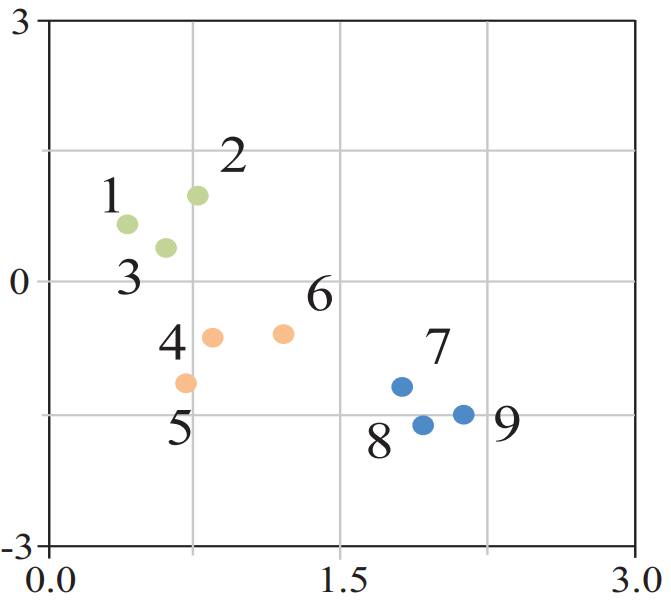
\includegraphics[width=7 cm]{images/graph_emb_2.png}
	\caption{
		Nhúng đỉnh với từng vector thể hiện đặc trưng của từng đỉnh}
	\label{fig:nodeEmbedding}
\end{figure}

Nhúng đỉnh (node embedding) biểu diễn mỗi đỉnh như một vector trong không gian số chiều thấp. Các đỉnh "gần" trong đồ thị được nhúng có các biểu diễn vector tương tự nhau. Sự khác biệt giữa các phương pháp nhúng đồ thị khác nhau nằm ở cách chúng xác định "độ gần nhau" giữa hai đỉnh. Lân cận bậc nhất (Định nghĩa \ref{def:firstOrderProximity}) và lân cận bậc hai (Định nghĩa \ref{def:secondOrderProximity})) là hai số liệu thường được sử dụng để tính độ tương tự đỉnh theo cặp. Trong một nghiên cứu, sự gần nhau bậc cao cũng được khám phá ở một mức độ nhất định. Ví dụ nắm bắt các quan hệ hàng xóm k-step (k = 1, 2, 3, ···) trong quá trình nhúng của chúng được đề cập trong nghiên cứu của nhóm tác giả Cao, Shaosheng\cite{cao2015grarep}.

\textbf{Nhúng cạnh}
\label{sec:edgeEmbedding}

\begin{figure}[htp]
	\centering
	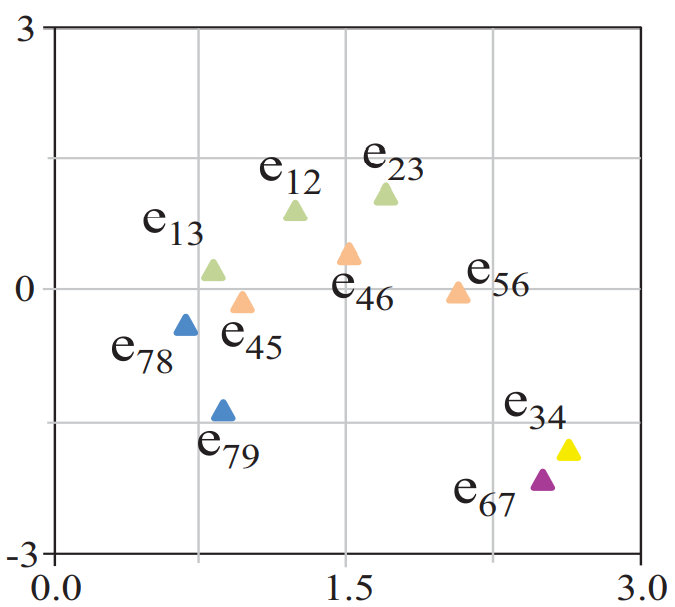
\includegraphics[width=7 cm]{images/graph_emb_3.png}
	\caption{Nhúng cạnh với từng vector thể hiện đặc trưng của từng cạnh}
	\label{fig:edgeEmbedding}
\end{figure}

Trái ngược với nhúng đỉnh, nhúng cạnh (edge embedding) nhằm mục đích biểu diễn một cạnh dưới dạng vector có số chiều thấp. Nhúng cạnh hữu ích trong hai trường hợp sau :

Thứ nhất, nhúng đồ thị tri thức. Mỗi cạnh là một bộ ba $\langle h, r, t \rangle$ (Định nghĩa \ref{def:knowledgeGraph}). Phép nhúng được học để bảo toàn r giữa h và t trong không gian nhúng, để một thực thể hoặc quan hệ bị thiếu có thể được dự đoán chính xác với hai thành phần còn lại trong $\langle h, r, t \rangle$.

Thứ hai, một số công việc nhúng một cặp đỉnh làm đặc trưng vector để làm cho cặp đỉnh này có thể so sánh với các đỉnh khác hoặc dự đoán sự tồn tại của một liên kết giữa hai đỉnh. Việc nhúng cạnh mang lại lợi ích cho việc phân tích đồ thị liên quan đến cạnh (cặp đỉnh), chẳng hạn như dự đoán liên kết, thực thể biểu diễn tri thức/dự đoán quan hệ, v.v.

\textbf{Nhúng Kết Hợp}

\begin{figure}[htp]
	\centering
	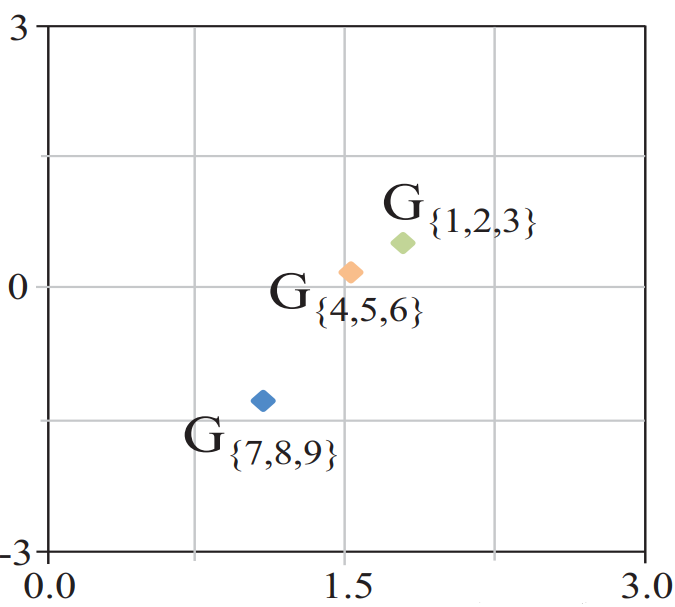
\includegraphics[width=6 cm]{images/graph_emb_4.png}
	\caption{Nhúng một cấu trúc bộ phận của đồ thị}
	\label{fig:substructureEmbedding}
\end{figure}

Nhúng kết hợp (hybrid embedding) là nhúng kết hợp các loại thành phần đồ thị khác nhau, ví dụ: đỉnh + cạnh (tức là cấu trúc con), đỉnh + bộ phận. Việc nhúng cấu trúc con hoặc bộ phận cũng có thể được bắt nguồn bằng cách tổng hợp các đỉnh riêng lẻ và nhúng cạnh bên trong nó. Tuy nhiên, kiểu tiếp cận "gián tiếp" như vậy không được tối ưu hóa để thể hiện cấu trúc của đồ thị. Hơn nữa, nhúng đỉnh và nhúng bộ phận có thể củng cố lẫn nhau. Nhúng đỉnh tốt hơn vì nó học được cách phối hợp từ sự quan tâm của nhóm lân cận bậc cao, nhúng bộ phận tốt hơn khi phát hiện chính xác hơn đỉnh nhúng được tạo ra.

\textbf{Nhúng Toàn Bộ Đồ Thị}

\begin{figure}[htp]
	\centering
	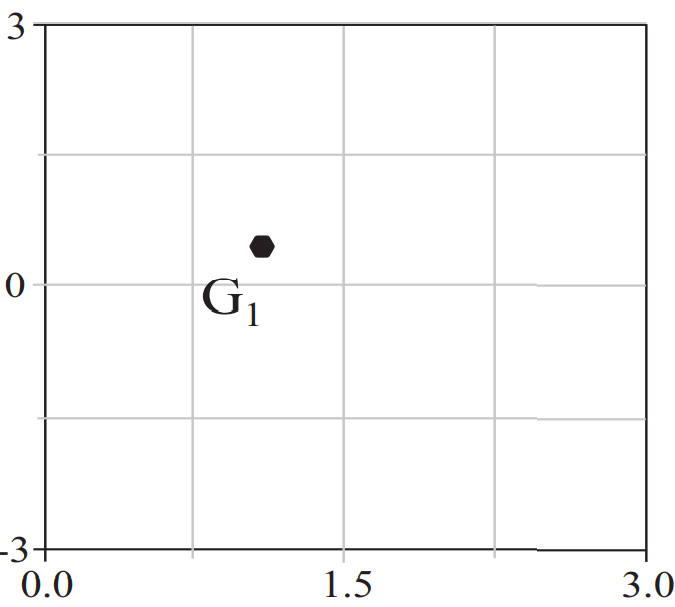
\includegraphics[width=6 cm]{images/graph_emb_5.png}
	\caption{Nhúng toàn bộ đồ thị}
	\label{fig:wholeGraphEmbedding}
\end{figure}

Nhúng toàn bộ đồ thị (whole-graph embedding) thường dành cho các đồ thị nhỏ, chẳng hạn như protein, phân tử, v.v. Trong trường hợp này, một đồ thị được biểu diễn dưới dạng một vector và hai đồ thị tương tự được nhúng để gần nhau hơn. Việc nhúng toàn bộ đồ thị mang lại lợi ích cho nhiệm vụ phân loại đồ thị bằng cách cung cấp một giải pháp đơn giản và hiệu quả để tính toán độ tương đồng của đồ thị. Để thiết lập sự thỏa hiệp giữa thời gian nhúng (tính hiệu quả) và khả năng lưu giữ thông tin (tính biểu đạt), phương pháp Nhúng đồ thị phân cấp \cite{mousavi2017hierarchical} thiết kế một khung nhúng đồ thị phân cấp. Nó cho rằng sự hiểu biết chính xác về thông tin đồ thị toàn cục đòi hỏi phải xử lý các cấu trúc con ở các quy mô khác nhau. Một kim tự tháp đồ thị được hình thành trong đó mỗi cấp là một đồ thị tóm tắt ở các tỷ lệ khác nhau. Biểu đồ được nhúng ở tất cả các cấp và sau đó được nối thành một vector. Việc nhúng toàn bộ đồ thị yêu cầu thu thâp được thông tin thuộc tính của toàn bộ đồ thị, và vì vậy sẽ tốn nhiều thời gian hơn các phương pháp thiết lập khác.

\subsection{Các kỹ thuật nhúng đồ thị}

\begin{figure}[htp]
	\centering
	\resizebox{\textwidth}{!}{
		\begin{tikzpicture}[
		rec/.style  = {draw, text width=2cm, font=\sffamily, rectangle, thin},
		root/.style = {rec, rounded corners=6pt, align=center, fill=green!60, text width=10em},
		level 1/.style={sibling distance=50mm},
		level 2/.style={rec, rounded corners=6pt, fill=green!30,align=center, text width=8em},
		level 3/.style = {rec, align=left, fill=pink!30, text width=8em, yshift=-20pt},
		edge from parent/.style={->,draw, very thick},
		>=latex]
		
		% root of the the initial tree, level 1
		\node[root] {Kỹ thuật nhúng đồ thị}
		% The first level, as children of the initial tree
		child {node[level 2] (c1) {Học sâu}}
		child {node[level 2] (c2) {Phân rã ma trận}}
		child {node[level 2] (c3) {Tái cấu trúc cạnh}}
		child {node[level 2] (c4) {Đồ thị lõi}}
		child {node[level 2] (c5) {Mô hình sinh}};
		
		% The second level, relatively positioned nodes
		\begin{scope}[every node/.style={level 3}]
		\node [below of = c1, xshift=30pt] (c11) {Sử dụng bước ngẫu nhiên};
		\node [below of = c11] (c12) {Không sử dụng bước ngẫu nhiên};
		
		\node [below of = c2, xshift=30pt] (c21) {Đồ thị toán tử Laplace Eigenmaps};
		\node [below of = c21] (c22) {Phân rã ma trận bằng xấp xỉ đỉnh};
		
		\node [below of = c3, xshift=25pt] (c31) {Cực đại hóa xác xuất tái cấu trúc cạnh};
		\node [below of = c31, yshift=-20pt] (c32) {Tối thiểu hóa mất mát dựa trên khoảng cách};
		\node [below of = c32, yshift=-20pt] (c33) {Tối thiểu hóa xếp hạng mất mát dựa trên lề};
		
		\node [below of = c4, xshift=25pt] (c41) {Dựa trên graphlet};
		\node [below of = c41] (c42) {Dựa trên mẫu nhánh cây};
		\node [below of = c42] (c43) {Dựa trên bước nhảy ngẫu nhiên};
		
		\node [below of = c5, xshift=30pt] (c51) {Nhúng đồ thị dựa trên không gian ẩn};
		\node [below of = c51] (c52) {Nhúng kết hợp ngữ nghĩa};
		\end{scope}
		
		% lines from each level 1 node to every one of its "children"
		\foreach \value in {1,2}
		\draw[->, very thick] (c1.195) |- (c1\value.west);
		
		\foreach \value in {1, 2}
		\draw[->, very thick] (c2.195) |- (c2\value.west);
		
		\foreach \value in {1,...,3}
		\draw[->, very thick] (c3.195) |- (c3\value.west);
		
		\foreach \value in {1,...,3}
		\draw[->, very thick] (c4.195) |- (c4\value.west);
		
		\foreach \value in {1,...,2}
		\draw[->, very thick] (c5.195) |- (c5\value.west);
		\end{tikzpicture}
	}
	\caption{Các kỹ thuật nhúng đồ thị}
	\label{fig:graphEmbeddingTechniquesTree}
\end{figure}

Trong phần này, chúng tôi phân loại các nhóm phương pháp nhúng đồ thị dựa vào kỹ thuật sử dụng, như đã nói ở trên, mục tiêu của việc nhúng đồ thị là biểu diễn một đồ thị vào không gian có số chiều thấp mà vẫn giữ vững được những thông tin vốn có của đồ thị nhiều nhất có thể. Các kỹ thuật nhúng đồ thị cơ bản khác nhau ở định nghĩa các đặc tính vốn có cần được đảm bảo. Vì mục tiêu chính của chúng tôi là tìm hiểu về các nhóm phương pháp nhúng đồ thị dựa trên kỹ thuật học sâu nên chúng tôi chỉ trình bày sơ lược đối với các nhóm phương pháp khác.

\textbf{Học sâu}

Ở phần này chúng tôi sẽ trình bày chi tiết về các hướng nghiên cứu của kỹ thuật học sâu (deep learning) bao gồm : sử dụng bước nhảy ngẫu nhiên (random walk) và không sử dụng bước nhảy ngẫu nhiên. Kỹ thuật học sâu được sử dụng phổ biến trong việc nhúng đồ thị bởi vì sự nhanh chóng và hiệu quả trong việc thu thập các đặc trưng một cách tự động. Trong các phương pháp sử dụng kỹ thuật học sâu này, cả 3 loại phương pháp thiết lập đồ thị dựa trên đầu vào (ngoại trừ đồ thị cấu trúc từ dữ liệu phi-quan hệ) và 4 loại đầu ra (Hình \ref{fig:graphEmbeddingSettingTree}) đều có thể áp dụng kỹ thuật học sâu. 

\textit{Kỹ thuật học sâu với bước nhảy ngẫu nhiên}

Trong nhóm phương pháp này, lân cận bậc hai (Định nghĩa \ref{def:secondOrderProximity}) trong đồ thị sẽ được bảo đảm trong không gian nhúng bằng cách cực đại hóa xác xuất của những hàng xóm quan sát của một đỉnh điều kiện trên vector nhúng của nó. Đồ thị sẽ được biểu diễn như là một tập hợp mẫu bằng cách lấy mẫu từ những bước đi ngẫu nhiên, và sau đó các phương pháp học sâu sẽ được áp dụng vào đồ thị nhúng để vẫn đảm bảo đặc tính của đồ thị mang theo thông tin đường đi. Các phương pháp sử dụng nhóm phương pháp này như : Deep Walk \cite{perozzi2014deepwalk}, LINE \cite{tang2015line}, Node2Vec \cite{grover2016node2vec}, Anonymous Walk \cite{ivanov2018anonymous}, NetGAN \cite{bojchevski2018netgan}, ...

\textit{Kỹ thuật học sâu không sử dụng bước nhảy ngẫu nhiên}

Trong phương pháp này, những cấu trúc học đa lớp sẽ được áp dụng một cách nhanh chóng và hiệu quả để biến đổi đồ thị thành không gian số chiều thấp hơn. Phương pháp này sẽ áp dụng cho toàn bộ đồ thị, có một số phương pháp phổ biến hiện nay đã được khảo sát và trình bày ở báo cáo \cite{rossi2020knowledge} như sau :

\begin{itemize}
	\item Mạng Neural Tích Chập (Convolutional Neural Networks)
	
	Mô hình này sử dụng nhiều lớp tích chập : Với mỗi lớp thực hiện tính tích chập trên dữ liệu đầu vào một bộ lọc có số chiều thấp. Kết quả là một ánh xạ đặc trưng, sau đó lại tiếp tục đi qua một lớp kết nối đầy đủ để tính giá trị xác xuất. Ví dụ như \textbf{ConvE} \cite{dettmers2017convolutional} : Mỗi thực thể và mối quan hệ sẽ được biểu diễn bằng một vector số chiều thấp $d-\text{chiều}$. Với mỗi bộ ba, nó ghép và thay đổi kích thước của vector nhúng đỉnh $h$ và quan hệ $r$ vào một đầu vào duy nhất $[h, r]$ với kích thước kết quả là $d_m \times d_n$. Sau đó nó đi qua lớp tích chập với bộ lọc $\omega$ có kích thước $m \times n$, rồi đi qua một lớp kết nối đầy đủ  (fully connected layers) và các trọng số $W$. Kết quả cuối cùng được kết hợp với vector nhúng đuôi $t$ bằng cách sử dụng tích vô hướng (dot products). Kiến trúc này có thể coi là một kiến trúc \textit{phân loại các lớp} .
	
	Một mô hình phổ biến khác là \textbf{ConvKB} \cite{nguyen2017novel}, tương tự như ConvE, nhưng nó ghép cả ba vector nhúng $h$, $r$ và $t$ vào một ma trận $[h, r, t]$ kích thước $d \times 3$ chiều. Sau đó nó đi qua một lớp tích chập với $T$ bộ lọc $\omega$ kích thước $1 \times 3$. Kết quả là $T \times 3$ ánh xạ đặc trưng. Sau đó ánh xạ đặc trưng lại đi qua lớp kết nối đầy đủ và trọng số $\mathbf{W}$. Kiến trúc này có thể coi là kiến trúc phân loại nhị phân.
	
	\item Mạng Hồi Qui Tuyến Tính (Recurrent Neural Networks)
	
	Những mô hình này sẽ cho một lớp hoặc nhiều lớp hồi tuyến tính để phân tích toàn bộ đường đi (một chuỗi sự kiện/bộ ba) lấy ra từ tập huấn luyện, thay vì chỉ xử lý các sự kiện một cách riêng biệt. Ví dụ như RSN \cite{guo2019learning}, nhận thấy mô hình hồi quy tuyến tính truyền thống không phù hợp cho đồ thị, với mỗi lần thực hiện nó chỉ lấy thông tin của mối quan hệ mà không lấy thông tin của vector đỉnh của lần thực hiện trước đó. Vì vậy nó không xử lý rõ ràng sự luân chuyển các đường dẫn của các thực thể và quan hệ. Để giải quyết vấn đề này, họ đề xuất RSN (Recurrent Skipping Networks \cite{guo2019learning}) : với mỗi bước nhảy, nếu đầu vào là quan hệ, một trạng thái ẩn được cập nhật để tái sử dụng thêm vector đỉnh. Sau đó, kết quả đầu ra được nhân tích vô hướng với mỗi vector nhúng mục tiêu.
	
	\item Mạng Neural Bao Bọc (Capsule Neural Networks)
	
	Mạng bao bọc (capsule networks) sẽ sắp một nhóm neural lại với nhau gọi là viên nang \label{capsule}, mỗi viên nang này sẽ mã hóa những đặc trưng đặc biệt của đầu vào, như là đại diện cho một nhóm hình ảnh cụ thể. Ưu điểm của mạng bao bọc đó là giúp nhận ra những đặc trưng mà không mất thông tin không gian so với việc tính tích chập thông thường. Mỗi một viên nang tìm ra những đặc trưng theo kích thước vector đầu ra. Ví dụ như : \textbf{CapsE} \cite{vu2019capsule}, mỗi thực thể và quan hệ được xem là một vector nhúng như trên, tương tự như ConvKB, nó sẽ ghép ba vector nhúng $h$, $r$ và $t$ thành một ma trận nhúng kích thước $d \times 3$. Sau đó nó đi qua lớp có E bộ lọc tích chập có kích thước $1 \times 3$. Kết quả là một ma trận kích thước $d \times E$ mà với mỗi dòng thứ $i-th$ đại diện cho những thực thể $h[i]$, $t[i]$ và quan hệ $r[i]$ riêng biệt. Ma trận này sẽ đi lớp bao bọc mà mỗi viên nang (\ref{capsule}) riêng biệt xử lý mỗi cột, vì vậy nó nhận được thông tin dựa theo một đặc trưng của bộ ba đầu vào. Và lớp thứ hai với một lớp bao bọc được sử dụng để đưa ra kết quả đầu ra.
	
	\item Mạng đồ thị chú ý (Graph Attention Networks)
	
	Nhóm phương pháp này sử dụng cơ chế chú ý (attention mechanism \cite{vaswani2017attention}) mà đã đạt được kết quả cải thiện đáng kể trong xử lý ngôn ngữ tự nhiên. Ở nhóm phương pháp này với mỗi vector nhúng, các thực thể được tổng hợp thông tin chú ý từ các thực thể kế cận, sau đó các thông tin chú ý được ghép chồng với nhau và đi qua một lớp kết nối đầy đủ và trọng số để biến đổi thành các vector nhúng cuối cùng. Ví dụ như : GAT \cite{velivckovic2017graph} với mỗi bộ ba từ tập huấn luyện được nhúng và áp dụng cơ chế chú ý đa đỉnh để cho ra một vector nhúng. Sau đó vector nhúng này tiếp tục đi qua một ma trận trọng số để biến đổi thành vector nhúng mới có số chiều lớn hơn tổng hợp thông tin từ các đỉnh kế cận từ bộ ba ban đầu. Một cải tiến khác của GAT bằng cách thêm thông tin của vector nhúng quan hệ là KBGAT \cite{nathani2019learning}. Các phương pháp này được trình bày cụ thể ở các phần tiếp theo.
	
	\item Ngoài ra còn một số phương pháp khác như sử dụng kỹ thuật tự động mã hóa (autoencoder) như Mạng Nhúng Cấu Trúc Sâu (Structural Deep Network Embedding \cite{wang2016structural}) .
\end{itemize}

\textbf{Phân rã ma trận}

Phân rã ma trận (matrix factorization) dựa trên đồ thị nhúng biểu diễn những đặc tính của đồ thị (ví dụ những cặp tương đồng hay giống nhau) dưới hình thức một ma trận và phân rã ma trận này để lấy được thông tin nhúng của đỉnh. Đầu vào của nhóm phương pháp này thường là những đặc trưng phi-quan hệ nhiều chiều và đầu ra là tập hợp các đỉnh nhúng. Có hai phương pháp nhúng đồ thị dựa trên phân rã ma trận bao gồm : Đồ Thị Toán Tử Laplace Eigenmaps (Graph Laplacian Eigenmaps) và Phân Rã Ma Trận Xấp Xỉ Đỉnh (Node Proximity Matrix Factorization)

\begin{itemize}
	\item \textit{Đồ Thị Toán Tử Laplace Eigenmaps}
	
	Nhóm phương pháp này sẽ đảm bảo đặc tính của đồ thị bằng cách phân tích những cặp tương đồng và sẽ phạt nặng những đỉnh có sự tương đồng lớn hơn mà nhúng xa nhau. 
	
	\item \textit{Phân Rã Ma Trận Xấp Xỉ Đỉnh}
	
	Nhóm phương pháp này sẽ xấp xỉ các đỉnh lân cận trong một không gian số chiều thấp sử dụng kỹ thuật phân rã ma trận. Mục tiêu là để bảo toàn những đỉnh lân cận để tối thiểu hóa hàm xấp xỉ.
\end{itemize}

\textbf{Tái cấu trúc cạnh}

Phương pháp tái cấu trúc cạnh (edge reconstruction) sẽ xây dựng các cạnh dựa trên những đỉnh nhúng sao cho giống với những đồ thị đầu vào nhất có thể. Phương pháp này tối tối đa hóa xác xuất tái tạo cạnh hoặc tối thiểu hóa hàm mất mát tái tạo cạnh, ngoài ra còn chia ra hàm mất mát dựa trên khoảng cách và hàm xếp hạng mất mất mát dựa trên lề .

\begin{itemize}
	\item \textit{Cực đại hóa xác xuất tái cấu trúc cạnh }
	
	Ở phương pháp Cực đại hóa xác xuất tái cấu trúc cạn (maximize edge reconstruct probability), một đỉnh nhúng tốt sẽ cực đại hóa xác xuất sinh của các cạnh quan sát trong một đồ thị. Nghĩa là một vector đỉnh nhúng tốt sẽ được tái xây dựng lại như là đồ thị đầu vào gốc. Chúng được phân biệt bằng cách cực đại hóa xuất xuất sinh của tất cả các cạnh quan sát sử dụng vector đỉnh nhúng .
	
	\item \textit{Tối thiểu hóa mất mát dựa trên khoảng cách}
	
	Trong phương pháp tối thiểu hóa mất mát dựa trên khoảng cách (minimize distance-based loss), các đỉnh lân cận tính toán dựa trên vector đỉnh nhúng phải càng gần nhất với những đỉnh lân cận trên các cạnh đang quan sát càng tốt.
	Cụ thể là, độ gần của đỉnh có thể được tính toán dựa trên những đỉnh nhúng hoặc được tính toán theo kinh nghiệm dựa trên các cạnh được quan sát. Sau đó sẽ được tối thiểu hóa sự khác biệt giữa hai loại lân cận để đảm bảo độ gần tương ứng.
	
	\item \textit{Tối thiểu hóa xếp hạng mất mát dựa trên lề}
	
	Trong phương pháp tối thiểu xếp hạng mất mát dựa trên lề (minimize margin-based ranking loss), các cạnh của đồ thị đầu vào thể hiện sự tương quan giữa những cặp đỉnh. Một số đỉnh trong đồ thị thì thường liên kết với những tập hợp đỉnh liên quan. Cụ thể phương pháp này sẽ giúp các đỉnh vector nhúng sẽ gần nhau nếu các đỉnh liên quan đến nhau hơn so với những đỉnh không liên quan khác.
\end{itemize}

\textbf{Đồ thị lõi}

Với đồ thị lõi (graph kernel) toàn bộ cấu trúc đồ thị có thể được biểu diễn như là một vector chứa số lượng cấu trúc con cơ bản được phân tách từ đồ thị. Kỹ thuật đồ thị lõi bao gồm các nhánh phương pháp con gồm : graphlet, mẫu đồ thị con (subtree patterns) và dựa trên bước nhảy ngẫu nhiên .

Phương pháp này được thiết kế để nhúng toàn bộ đồ thị chỉ lấy đặc trưng toàn cục của toàn bộ đồ thị. Đầu vào của phương pháp này thường là đồ thị đồng nhất. hoặc đồ thị với thông tin bổ trợ

\textbf{Mô hình sinh}

Một mô hình sinh (generative model) có thể được định nghĩa bằng cách xác định sư phân phối chung của đặc trưng đầu vào và những lớp nhãn, và được điều chỉnh dựa trên một tập những tham số. Có hai nhóm phương pháp con của mô hình sinh bao gồm : Nhúng đồ thị dựa trên không gian ẩn (embed graph into latent space) và nhúng kết hợp ngữ nghĩa (incorporate semantics for embedding).
Mô hình sinh có thể được dùng cho cả nhúng đỉnh và nhúng cạnh . Nó được xem như là đỉnh những ngữ nghĩa với đầu vào thường là các đồ thị không đồng nhất hoặc đồ thị với thông tin phụ trợ.
\begin{itemize}
	\item \textit{Nhúng đồ thị trên không gian ngữ nghĩa ẩn}
	
	Với nhóm phương này, các đỉnh được nhúng vào một không gian ngữ nghĩa ẩn nơi khoảng cách giữa cách đỉnh mô tả được cấu trúc của đồ thị.
	
	\item \textit{Nhúng kết hợp ngữ nghĩa}
	
	Phương pháp này thì mỗi đỉnh sẽ gần với đồ thị và có ngữ nghĩa mà nó phải được nhúng gần hơn. Những đỉnh ngữ nghĩa có thể được tìm ra từ những đỉnh mô tả thông qua một mô hình sinh.
	
\end{itemize}

\textbf{Tổng kết} : Các phương pháp nhúng đồ thị đều có ưu nhược điểm riêng được nhóm tác giả Cai, Hongyun\cite{cai2018comprehensive} tổng hợp và trình bày lại ở bảng \ref{tab:graphEmbeddingTechCompare}. Với nhóm phương pháp \textit{phân rã ma trận} dựa trên đồ thị nhúng sẽ học những đại diện dựa trên việc phân tích sự tương đồng các cặp toàn cục. Với nhóm phương pháp \textit{học sâu}, những mô hình này đạt được kết quả hứa hẹn so với những phương pháp khác và phù hợp cho việc nhúng đồ thị vì nó có khả năng học được các biểu diễn phức tạp từ các cấu trúc đồ thị phức tạp. Các phương pháp sử dụng kỹ thuật bước nhảy ngẫu nhiễn trong học sâu có chi phí tính toán thấp hơn so với các phương pháp sử dụng kỹ thuật học sâu. Các phương pháp truyền thống coi đồ thị như một lưới, tuy nhiên nó không giống với bản chất của đồ thị. Với nhóm phương pháp \textit{tái cấu trúc cạnh} sẽ tối ưu hàm mục tiêu dựa trên các cạnh quan sát hoặc xếp hạng các bộ ba. Nhóm phương pháp này hiệu quả hơn nhưng vector nhúng kết quả lại không quan tâm đến cấu trúc toàn cục của đồ thị. Nhóm phương pháp \textit{đồ thị lõi} chuyển đồ thị vào một vector để dễ dàng thực hiện các nhiệm vụ phân tích đồ thị như phân loại đồ thị. Vì vậy nó chỉ hiệu quả khi liệt kê những nhánh cấu trúc đơn vị mong muốn trong một đồ thị. Với nhóm phương pháp \textit{mô hình sinh}, nó tận dụng thông tin một cách tự nhiên từ nhiều nguồn khác nhau trong một mô hình duy nhất. Việc nhúng đồ thị vào không gian ngữ nghĩa ẩn tạo ra những vector nhúng có thể được diễn giải bằng cách sử dụng ngữ nghĩa. Nhưng giả định về việc lập mô hình quan sát bằng cách sử dụng các phân bố nhất định là khó có thể biện minh. Hơn nữa, phương pháp sinh cần một lượng lớn dữ liệu huấn luyện để ước tính mô hình kết quả phù hợp với dữ liệu. Vì thế nó có thể không đạt kết quả tốt cho những đồ thị nhỏ hoặc số lượng nhỏ đồ thị.
\newcolumntype{L}{>{\arraybackslash}m{5cm}}
\begin{table}[htbp]
	\begin{center}
		\resizebox{\textwidth}{!}{
			\begin{tabular}{|p{2cm}|L|L|L|}
				\hline
				Phương pháp & Danh mục con & Ưu điểm & Nhược điểm \\
				\hline \hline
				Phân rã ma trận & Đồ thị toán tử Laplace Eigenmap            & Xem xét toàn cục các đỉnh lân cận &
				Sử dụng không gian và thời gian tính toán lớn\\
				\cline{2-2}
				& Phân rã ma trận bằng xấp xỉ đỉnh & & \\
				\hline
				\multirow{3}{2cm}{Tái cấu trúc cạnh} & Cực đại hóa xác xuất tái cấu trúc cạnh & \multirow{3}{5cm}{Huấn luyện tương đối hiệu quả} & \multirow{3}{5cm}{Tối ưu chỉ sử dụng thông tin cục bộ. Ví dụ như các cạnh (hàng xóm 1 nước) hoặc cặp đỉnh xếp hạng } \\ \cline{2-2}
				& Tối thiểu hóa mất mát dựa trên khoảng cách & & \\ \cline{2-2}
				& Tối thiểu hóa xếp hạng mất mát dựa trên lề & & \\ \hline
				\multirow{3}{2cm}{Đồ thị lõi} & Dựa trên graphlet & Hiệu quả, chỉ tính những nhánh cấu trúc đơn vị mong muốn & \multirow{3}{5cm}{Nhánh cấu trúc thì không độc lập. Số chiều nhúng tăng lên theo hàm mũ} \\ \cline{2-2}
				& Dựa trên mẫu nhánh cây   & & \\ \cline{2-2}
				& Dựa trên bước nhảy ngẫu nhiên & & \\ \hline
				
				Mô hình sinh & Nhúng đồ thị dựa trên không gian ẩn & Phép nhúng có thể giải thích được & Khó điều chỉnh lựa chọn phân bố \\ \cline{2-3}
				
				& Nhúng kết hợp ngữ nghĩa & Tận dụng nhiều thông tin nguồn & Yêu cầu một lượng lớn dữ liệu huấn luyện\\
				& & một cách tự nhiên & \\ \hline
				
				Học sâu & Sử dụng bước ngẫu nhiên & \multirow{2}{5cm}{Hiệu quả và nhanh chóng Không phải trích đặc trưng} & Chỉ xem xét đến nội dung cục bộ trong một đường đi. Khó để tìm kiếm chiến lược lấy mẫu tối ưu \\ \cline{2-2} \cline{4-4} 
				& Không sử dụng bước ngẫu nhiên &  & Chi phí tính toán cao \\ \hline
			\end{tabular}
		}
		\caption{Bảng so sánh ưu và nhược điểm của kỹ thuật nhúng đồ thị}
		\label{tab:graphEmbeddingTechCompare}
	\end{center}
\end{table}

Trong các phương pháp trên, nhóm phương pháp nhúng đồ thị bằng học sâu giúp học được các biểu diễn phức tạp và đạt được kết quả hứa hẹn nhất hiện nay. Tuy nhiên, nhược điểm của nhóm phương pháp học sâu đối với nhúng đồ thị là nếu coi các đỉnh và cạnh trong đồ thị như một lưới để thực hiện tích chập thì sẽ không đúng với bản chất của đồ thị vì không đảm bảo cấu trúc không gian của đồ thị. Mô hình mạng chú ý trên đồ thị dựa trên cơ chế chú ý giúp tổng hợp thông tin của một thực thể dựa vào các trọng số chú ý của các thực thể lân cận đối với thực thể gốc. Chúng tôi cho rằng đây là hướng nghiên cứu tương tự như quan hệ giữa chú ý và ghi nhớ \cite{memoryandattention:2020}, sự phân bố của chú ý sẽ quyết định trọng số hay sự quan trọng của một thực thể này đối với một thực thể khác. Cũng như vector nhúng biểu diễn cho một thực thể sẽ bị ảnh hưởng bởi sự chú ý hay sự quan trọng của các vector nhúng lân cận. Vì vậy đây là hướng nghiên cứu chúng tôi chọn trong các nhóm phương pháp trên.

%
%Trong cơ chế chú ý, khi nhân các vector
%

\section{Cơ chế chú ý đa đỉnh}

Năm 2014, cơ chế chú ý đa đỉnh (multi-head attention) được phát minh bởi nhóm tác giả Bahdanau, Dzmitry\cite{bahdanau2014neural} nhưng mãi đến năm 2017 nó mới được phổ biến thông qua mô hình Transformer của nhóm tác giả Vaswani, Ashish\cite{vaswani2017attention}. Cơ chế chú ý là một phương pháp hiệu quả giúp thể hiện sự quan trọng của một từ với các từ khác trong một câu, nó còn được chứng minh là đại diện cho bất kỳ phép tính tích chập nào trong báo cáo của nhóm tác giả Cordonnier, Jean-Baptiste\cite{cordonnier2019relationship}. Để hiểu về cách cơ chế chú ý đa đỉnh được áp dụng vào trong đồ thị, trong phần này chúng tôi sẽ trình bày lại chi tiết về cơ chế chú ý đa đỉnh cũng như cải tiến mới nhất của cơ chế chú ý đa đỉnh của nhóm tác giả Cordonnier, Jean-Baptiste\cite{cordonnier2020multi}
%
%trong phần này chúng tôi sẽ trình bày chi tiết về cơ chế chú ý đa đỉnh cũng như cải tiến mới nhất trên cơ chế chú ý đa đỉnh \cite{cordonnier2020multi} được chúng tôi gọi là \textit{cộng tác đa đỉnh chú ý} (collaborate multi-head attention).

\subsection{Cơ Chế Chú Ý (Attention Mechanism)}
\label{sec:attentionMechanism}

Ta gọi $\mathbf{X} = \Big\{\overrightarrow{x_1}, \overrightarrow{x_2}, ...,  \overrightarrow{x_{N_x}}\Big\}$ và $\mathbf{Y} = \Big\{\overrightarrow{y_1}, \overrightarrow{y_2}, ...,  \overrightarrow{y_{N_y}}\Big\}$ là các ma trận nhúng đầu vào, với mỗi dòng $i^{\text{th}}$ hay $j^{\text{th}}$ trong ma trận $\mathbf{X}$ hay $\mathbf{Y}$ là một vector nhúng $\overrightarrow{x_i} \in \mathbb{R}^{1 \times D_{\text{in}}}$, $\overrightarrow{y_j} \in \mathbb{R}^{1 \times D_{\text{in}}}$.
Cơ chế chú ý là quá trình biến đổi vector có $D_{\text{in}}$ chiều thành vector đầu ra có $D_{\text{attention}}$ chiều để thể hiện sự quan trọng của từng $N_x$ phần tử $x$ so với tất cả $N_y$ các phần tử $y$. Với $\mathbf{X} \in \mathbb{R}^{N_x \times D_\text{in}}$ và $\mathbf{Y} \in \mathbb{R}^{N_y \times D_\text{in}}$ là các ma trận nhúng đầu vào, và $\mathbf{H} \in \mathbb{R}^{N_x \times D_\text{attention}}$ là ma trận nhúng đầu ra như công thức sau :

\begin{equation}
\label{attention}
\mathbf{H} = \text{Attention}(\mathbf{Q}, \mathbf{K}, \mathbf{V}) = \text{softmax}\Big(\frac{\mathbf{Q}\mathbf{K}^T}{\sqrt{d_k}}\Big) \mathbf{V}
\end{equation}

với  $\mathbf{Q} = \mathbf{X}\mathbf{W}_Q, \mathbf{K} = \mathbf{Y} \mathbf{W}_K, \mathbf{V} = \mathbf{Y} \mathbf{W}_V$

Các ma trận trọng số 
$\mathbf{W}_Q \in \mathbb{R}^{D_{\text{in}} \times D_{k}}$, 
$\mathbf{W}_K \in \mathbb{R}^{D_{\text{in}} \times D_{k}}$ và 
$\mathbf{W}_V \in \mathbb{R}^{D_{\text{in}} \times D_{\text{attention}}}$ là các ma trận thể hiện quá trình tham số hóa để biến đổi các vector nhúng đầu vào $D_{\text{in}}$ chiều thành vector nhúng đầu ra có $D_{k}$ hoặc $D_{\text{attention}}$ chiều. $\mathbf{Q}\mathbf{K}^T$ là quá trình nhân tích vô hướng của từng vector nhúng $x$ ban đầu với tất cả vector nhúng y. Việc chia cho $\sqrt{d_k}$ là để chuẩn hóa theo số chiều $k$. Sau đó kết quả được chuẩn hóa lại bằng hàm \textit{softmax} để thể hiện độ lớn xác xuất của từng giá trị chú ý đối với phần tử x. Cuối cùng, kết quả được nhân với vector nhúng $\mathbf{V}$ để biến đổi từ vector nhúng $D_{k}$ chiều thành vector nhúng mới  $D_{\text{attention}}$ chiều .

Nếu $\mathbf{X} = \mathbf{Y}$ nghĩa là chúng ta đang tính sự quan trọng của một phần tử so với chính các phần tử khác trong ma trận nhúng ban đầu và ta gọi nó là cơ chế tự-chú ý (self-attention mechanism) .

\subsection{Chú Ý Đa Đỉnh (Multi-Head Attention)}

Tương tự như cơ chế chú ý ở trên, cơ chế chú ý đa đỉnh (multi-head attention mechanism) là quá trình biến đổi $N_x$ vector nhúng ban đầu $D_{\text{in}}$ chiều thành vector nhúng $D_{\text{multi-head}}$ chiều với thông tin được tổng hợp từ nhiều đỉnh khác nhau giúp ổn định trong quá trình huấn luyện. Cơ chế chú ý đa đỉnh sẽ ghép $N_{\text{head}}$ các đầu ma trận chú ý $\mathbf{H}$ rồi sau đó tiếp tục nhân với một ma trận trọng số để biến đổi từ ma trận nhúng $\mathbf{X} \in \mathbb{R}^{N_x \times D_\text{in}}$ ban đầu thành ma trận nhúng mới $\mathbf{X}' \in \mathbb{R}^{N_x \times D_{\text{multi-head}}}$ như công thức sau :

\begin{equation}
\label{headAttention}
\begin{split}
\mathbf{X}'& =\left(\bigparallel_{h=1}^{N_{\text{head}}}\mathbf{H}^{(h)}\right)\mathbf{W}^{O} \\
& = \left(\bigparallel_{h=1}^{N_{\text{head}}} \text{Attention}(\mathbf{X} \mathbf{W}_Q^{(h)}, \mathbf{Y} \mathbf{W}_K^{(h)}, \mathbf{Y} \mathbf{W}_V^{(h)}) \right)\mathbf{W}^{O}
\end{split}
\end{equation}

Trong đó các ma trận trọng số $\mathbf{W}_Q^{(h)}$, $\mathbf{W}_K^{(h)} \in \mathbb{R}^{D_{\text{in}} \times D_{k}}$ và $\mathbf{W}_V^{(h)} \in \mathbb{R}^{D_{\text{in}} \times D_{\text{attention}}}$ thuộc vào từng lớp chú ý $h \in [N_{\text{head}}]$ khác nhau. $\mathbf{W}^{O} \in \mathbb{R}^{N_{\text{head}} D_{\text{attention}} \times D_{\text{multi-head}}}$ để tham số hóa quá trình biến đổi ma trận các đỉnh đã ghép thành một ma trận nhúng kết quả cuối cùng.

\textbf{Lớp cộng tác đa đỉnh chú ý}

\cite{weng2018attention}

\section{Mạng đồ thị chú ý}
\label{sec:GAT}

\definecolor{amber}{rgb}{1.0, 0.75, 0.0}
\definecolor{azure}{rgb}{0.0, 0.5, 1.0}
\definecolor{awesome}{rgb}{1.0, 0.13, 0.32}
\begin{figure}[htp]
	\centering
	\resizebox{\textwidth}{!}{%
		\begin{tikzpicture}[
		entityStyle/.style={draw, color=white, font=\sffamily, thin, align=center, circle, text width=20mm},
		us/.style = {entityStyle, fill=amber},
		entity/.style={entityStyle, fill=azure},
		arrowStyle/.style={-latex', >=stealth, font=\sffamily}]
		
		\node[us] (us) {\textbf{U.S}};
		
		\begin{scope}[every node/.style={entity}]
		\node[above left=2cm of us, xshift=-20mm] (c1) {\textbf{Donald Trump}};
		\node[above right=2cm of us, xshift=1cm] (c2) {\textbf{Jeff Bezos}};
		\node[below left=2cm of us, xshift=-20mm] (c3) {\textbf{New York}};
		\node[below right=2cm of us, xshift=1cm] (c4) {\textbf{Tesla Inc.}};
		
		\node[below left=3cm of c1, yshift=25mm, xshift=-15mm] (c1x) {\textbf{Melania Trump}};
		\node[above left=3cm of c3, yshift=-25mm, xshift=-15mm] (c3x) {\textbf{Tom Cruise}};
		\end{scope}
		\foreach \value in {1,...,4}
		\draw[->, line width=0.8mm, azure] (c\value) -> (us);
		\foreach \value in {1,3}
		\draw[->, line width=0.8mm, azure] (c\value x) -> (c\value);
		
		\foreach \value in {1,3}
		\draw[->, line width=0.8mm, azure!60, dash pattern=on 3mm off 1mm, postaction={decorate}] (c\value x) -> (us);
		
		\path[arrowStyle] (c1)--node[rotate=-31, yshift=4mm]{president\_of} node[rotate=-31, yshift=-3mm]{$\alpha_{i4}$} (us);
		
		\path[arrowStyle] (c3)--node[rotate=30, yshift=4mm]{state\_of} node[rotate=30, yshift=-4mm]{$\alpha_{i3}$} (us);
		
		\path[arrowStyle] (c2)--node[rotate=41, yshift=4mm]{richest\_of} node[rotate=41, yshift=-4mm]{$\alpha_{i1}$} (us);
		
		\path[arrowStyle] (c4)--node[rotate=-41, yshift=4mm]{founded\_in} node[rotate=-41, yshift=-4mm]{$\alpha_{i2}$} (us);
		
		\path[arrowStyle] (c1x)--node[rotate=15, yshift=4mm]{wife\_of} (c1);
		\path[arrowStyle] (c3x)--node[rotate=-15, yshift=4mm]{born\_in} (c3);
		
		\path[arrowStyle] (c1x)--node[rotate=-8, yshift=4mm]{\textbf{first\_lady}} node[rotate=-8, yshift=-3mm]{$\alpha_{i5}$} (us);
		\path[arrowStyle] (c3x)--node[rotate=8, yshift=4mm]{\textbf{native\_of}} node[rotate=8, yshift=-3mm]{$\alpha_{i6}$} (us);
		\end{tikzpicture}
	}
	\caption{Đồ thị tri thức và các hệ số chú ý chuẩn hóa của thực thể}
	\label{fig:graphExample}
\end{figure}

Với thành công của \textit{cơ chế chú ý đa đỉnh} trong ngôn ngữ tự nhiên, nó còn được nghiên cứu để áp dụng vào các mô hình của xử lý ảnh \cite{ramachandran2019stand}. Chính vì vậy cơ chế chú ý đa đỉnh đã được nghiên cứu để áp dụng vào các mô hình nhúng đồ thị tri thức thay cho một phương pháp tính chập như Mạng Đồ Thị Tích Chập (GCNs \cite{kipf2016semi}). Ở phần này chúng tôi sẽ trình bày chi tiết về cách cơ chế chú ý ở \ref{sec:attentionMechanism} được áp dụng vào việc nhúng đồ thị theo phương pháp Mạng Đồ Thị Chú Ý (Graph Attention Network - GAT \cite{velivckovic2017graph}).

Đầu vào của mô hình \textit{mạng đồ thị chú ý} là tập hợp các vector nhúng được khởi tạo ngẫu nhiên theo phân phối chuẩn biểu diễn đặc trưng của từng thực thể (entity) trong không gian : $\mathbf{E} = \Big\{\overrightarrow{e_1}, \overrightarrow{e_2}, ...,  \overrightarrow{e_{N_e}}\Big\}$. Mục tiêu của mô hình là biến đổi thành ma trận nhúng đầu ra mới $\mathbf{E}'' = \Big\{\overrightarrow{e''_1}, \overrightarrow{e''_2}, ...,  \overrightarrow{e''_{N_e}}\Big\}$ với khả năng tổng hợp thông tin nhúng từ các thực thể lân cận; $\mathbf{E} \in \mathbb{R}^{N_e \times D_{\text{in}}}$ và $\mathbf{E}'' \in \mathbb{R}^{N_e \times D''}$ tương ứng là ma trận nhúng đầu vào và ma trận nhúng đầu ra của của tập hợp thực thể, $N_e$ là kích thước của tập thực thể, $D_{\text{in}}$ và $D''$ tương ứng là số chiều nhúng đầu vào, và số chiều nhúng đầu ra

Tương tự như cơ chế chú ý đa đỉnh được trình bày ở mục \ref{sec:attentionMechanism}, việc áp dụng của cơ chế chú ý đa đỉnh trên đồ thị tri thức sẽ áp dụng với chính mỗi vector nhúng thực thể giống như \textit{cơ chế tự-chú ý} (self-attention mechanism), mỗi đỉnh sẽ chú ý với tất cả các đỉnh khác trong đồ thị. Tuy nhiên, việc tính hệ số chú ý giữa tất cả các đỉnh với nhau trong đồ thị là không có ý nghĩa nếu không có mối quan giữa chúng và khối lượng tính toán rất lớn, vì vậy mô hình áp dụng cơ chế gọi là \textit{mặt nạ chú ý} (mask attention) bằng cách bỏ đi tất cả những hệ số chú ý không có quan hệ trong đồ thị, đó chính xác là giá trị của lân cận bậc nhất (Định nghĩa \ref{def:firstOrderProximity}) của một đỉnh trong đồ thị. Khi đó $\mathbf{X} = \mathbf{Y} = \mathbf{E}$ (\ref{sec:attentionMechanism}) và hệ số chú ý của của cơ chế mặt nạ chú ý được hiểu là sự quan trọng của một đỉnh $j \in \mathcal{N}_{i}$ đối với đỉnh gốc $i$, với $\mathcal{N}_{i}$ là tập hợp tất cả những hàng xóm của đỉnh $i$ (bao gồm cả $i$). 

Việc áp dụng cơ chế chú ý đa đỉnh (\textit{multi-head attention}) ở \ref{headAttention} vào đồ thị được mô tả như sau :

\begin{equation}
\label{maskAttention}
\centering
{e_{ij}}={f_{\text{mask attention}}(\mathbf{W} \overrightarrow{e_i}, \mathbf{W} \overrightarrow{e_j})}
\end{equation}

trong đó $e_{ij}$ là hệ số chú ý đa đỉnh của một cạnh $(e_i, e_j)$ đối với thực thể gốc $e_i$ trong đồ thị $\mathcal{G}_{\text{know}}$. $\mathbf{W}$ là ma trận trọng số để tham số hóa quá trình biến đổi tuyến tính. $f_{\text{mask attention}}$ là hàm áp dụng cơ chế chú ý.

Trong mô hình GAT, mô hình sẽ đi qua hai quá trình biến đổi vector nhúng $\overrightarrow{e_i}$ của thực thể $e_i$. Toàn bộ mô hình bao gồm hai bước biến đổi, với mỗi bước là một quá trình biến đổi vector nhúng bằng cơ chế chú ý đa đỉnh như sau :
\begin{equation}
\label{gatProcess}
\overrightarrow{e_i} \xrightarrow{f_{\text{mask attention}}^{(1)}} \overrightarrow{e'_i} \xrightarrow{f_{\text{mask attention}}^{(2)}} \overrightarrow{e''_i}
\end{equation}

Ở quá trình chú ý đa đỉnh đầu tiên ($f_{\text{mask attention}}^{(1)}$), mô hình sẽ tổng hợp thông tin từ các thực thể lân cận và ghép chồng lên nhau để tạo ra vector $\overrightarrow{e'_i}$, với $\overrightarrow{e'_i} \in \mathbb{R}^{1 \times D'}$ . Ở bước thứ hai ($f_{\text{mask attention}}^{(2)}$), lớp chú ý đa đỉnh đã đỉnh không còn nhạy cảm với quá trình tự-chú ý nên kết quả sẽ được tính \textit{trung bình} thay vì ghép các đỉnh chú ý lại với nhau, vector $\overrightarrow{e'_i}$ tiếp tục được xem là vector nhúng đầu vào để biến đổi thành vector nhúng $\overrightarrow{e''_i}$ cuối cùng với $\overrightarrow{e''_i} \in \mathbb{R}^{1 \times D''}$.

Đầu tiên, giống như cơ chế chú ý \ref{attention}, mỗi vector nhúng sẽ được nhân với một ma trận trọng số $\mathbf{W}_1 \in \mathbb{R}^{D_k \times D_{\text{in}}}$ để thể tham số hóa quá trình biến đổi tuyến tính từng vector nhúng của thực thể từ số chiều $D_{\text{in}}$ lên số chiều $D_k$ có đặc trưng cao hơn :

\begin{equation}
\overrightarrow{h_i} = \mathbf{W}_{1} \overrightarrow{e_i}
\end{equation}

khi đó $\overrightarrow{e_i} \in \mathbb{R}^{D_{\text{in}} \times 1}
\xrightarrow{} \overrightarrow{h_i} \in \mathbb{R}^{D_k \times 1}$

Sau đó, ta ghép các cặp vector nhúng thực thể vừa biến đổi tuyến tính với nhau để tính hệ số chú ý, hệ số chú ý $e_{ij}$ thể hiện sự quan trọng của đặc trưng cạnh $(e_i, e_j)$ đối với thực thể gốc $e_i$ hay sự quan trọng của một thực thể $e_j$ có quan hệ với thực thể gốc $e_i$ , ta áp dụng hàm $\text{LeakyReLU}$ để lấy giá trị tuyệt đối của hệ số chú ý, mỗi hệ số chú ý $e_{ij}$ được tính theo công thức sau :

\begin{equation}
e_{ij} = \Big( \text{LeakyReLU} \Big( \overrightarrow{\mathbf{W}_{2}}^{T} [\overrightarrow{h_i} || \overrightarrow{h_j}]\Big) \Big)
\end{equation}

với ${.}^{T}$ là phép chuyển vị, $||$ là phép ghép. Tương tự \ref{attention}, tuy nhiên thay vì thực hiện tính tích vô hướng thì ta sử dụng một \textit{cơ chế chú ý chung} (shared attentional mechanism) $\overrightarrow{\mathbf{W}_2}$ : $\mathbb{R}^{D_k} \times \mathbb{R}^{D_k} \xrightarrow{} \mathbb{R}$ để tính hệ số chú ý. Như đã trình bày ở \ref{maskAttention}, ta thực hiện tự chú ý giữa tất cả các đỉnh với nhau bằng cơ chế mặt nạ chú ý để bỏ hết tất cả thông tin cấu trúc.
Để có thể dễ dàng so sánh các hệ số chú ý với nhau giữa tất cả các thực thể, một hàm \textit{softmax} được áp dụng để chuẩn hóa trên tất cả các hàng xóm $e_j$ có quan hệ với thực thể gốc $e_i$ : $\alpha_{ij} = \text{softmax}_j(e_{ij})$. Kết hợp lại ta có công thức của hệ số chú ý chuẩn hóa của từng hàng xóm đối với thực thể gốc như sau :

\begin{equation}
\label{attentionCoeff}
\alpha_{ij} = \frac{
	\text{exp} \Big( \text{LeakyReLU} \Big( \overrightarrow{\mathbf{W}_2}^{T} [ \overrightarrow{h_i} || \overrightarrow{h_j}]\Big) \Big))
}
{
	\sum_{k \in \mathcal{N}_i}
	\text{exp} \Big( \text{LeakyReLU} \Big( \overrightarrow{\mathbf{W}_2}^{T} [\overrightarrow{h_i} || \overrightarrow{h_k}]\Big) \Big))
}
\end{equation}

Ở bước này, mô hình GAT tương tự như GCN \cite{kipf2016semi}, các vector nhúng từ hàng xóm sẽ được tổng hợp với nhau và mở rộng hay thu nhỏ (scale) theo hệ số chú ý đã chuẩn hóa :

\begin{equation}
\label{scaleAttentionCoef}
\centering
{\overrightarrow{e'_i}}={\sigma\left(\sum_{j\in \mathcal{N}_i} {\alpha_{ij} \overrightarrow{h_j} }\right)}
\end{equation}

Tương tự như lớp chú ý đa đỉnh, ta sẽ ghép $N_{\text{head}}$ đỉnh lại với nhau để giúp ổn định quá trình học ở bước ($f_{\text{mask attention}}^{(1)}$ \ref{gatProcess}) đầu tiên của mô hình:

\begin{equation}
\label{multiHeadAttention}
{\overrightarrow{e'_i}}={\bigparallel_{h=1}^{N_{\text{head}}}\sigma\left(\sum_{j\in \mathcal{N}_i}\alpha_{ij}^{h} \mathbf{W}^{h} \overrightarrow{h_{j}} \right)}
\end{equation}

trong đó $\sigma$ là bất kỳ hàm biến đổi phi tuyến tính nào, $\alpha_{ij}^h$ là hệ số chú ý được chuẩn hóa của cạnh $(e_i, e_j)$ được tính từ lớp thứ $h^{th}$, tương tự như công thức \ref{attention} $\mathbf{W}^h$ là ma trận trọng số để biến đổi tuyến tính vector nhúng đầu vào, với $\mathbf{W}^h$ thuộc các lớp ghép chồng $h^{th}$ khác nhau. Cuối cùng vector nhúng mới $\overrightarrow{e'_i} \in \mathbb{R}^{1 \times D'}$ với $D' = N_{\text{head}} D_{\text{k}}$ tiếp tục được xem là vector đầu vào để thực hiện cơ chế chú ý. Tuy nhiên ở bước thứ hai ($f_{\text{mask attention}}^{(2)}$ \ref{gatProcess}) giá trị chú ý đa đỉnh sẽ được tính trung bình thay vì ghép chồng lên nhau theo công công thức sau :

\begin{equation}
\label{multiHeadConcat}
{\overrightarrow{e''_i}}={\sigma\left(\frac{1}{N_{\text{head}}} \sum_{h=1}^{N_{\text{head}}}\sum_{j\in \mathcal{N}_i}\alpha_{ij}^{h} \mathbf{W}^{h} \overrightarrow{e'_{j}} \right)}
\end{equation}

\textbf{Tổng kết} : Đến đây chúng tôi đã trình bày được cách cơ chế chú ý tổng hợp một vector nhúng thực thể trong đồ thị tri thức từ các vector nhúng lân cận và ghép lại với nhau để tạo ra vector nhúng kết quả. Trong phần tiếp theo chúng tôi sẽ trình bày đầy đủ về mô hình nhúng của chúng tôi dựa trên mô hình KBGAT của nhóm tác giả Nathani, Deepak\cite{nathani2019learning} .

\section{Mô hình KBGAT}

Trong đồ thị tri thức, một thực thể không thể là một đại diện đầy đủ cho một cạnh, vì một thực thể có thể đóng nhiều vai trò khác nhau phụ thuộc vào từng loại quan hệ khác nhau. Ví dụ như hình \ref{fig:graphExample}, Donald Trump vừa đóng là vai trò là tổng thống, vừa đóng vai trò là người chồng. Để giải quyết vấn đề này, mô hình nhúng đồ thị dựa trên chú ý - KBGAT (graph attention based embeddings \cite{nathani2019learning}) là một cải tiến của mô hình GAT bằng cách kết hợp thêm thông tin của \textit{quan hệ và đặc trưng các đỉnh hàng xóm} vào trong cơ chú ý. Trong phần này chúng tôi sẽ trình bày chi tiết về mô hình KBGAT.

\begin{equation}
\label{eq:KBGATProcess}
entities \xrightarrow{\text{Embedding}^{\ref{sec:initTransE}}} \overrightarrow{e_{\text{TransE}}} \xrightarrow{\text{Embedding} ^{\ref{sec:encodeKBGAT}}} \overrightarrow{e_{\text{KBGAT}}} \xrightarrow{\text{ConvKB}^{\ref{sec:predictionConvKB}}} e_{\text{prob}}
\end{equation}

Các bước của mô hình KBGAT được minh họa ở \ref{eq:KBGATProcess}. Đầu tiên, các vector nhúng của mỗi thực thể được khởi tạo bằng mô hình TransE để học được các đặc trưng không gian giữa các thực thể để thu được vector nhúng. Sau đó các vector nhúng này được nhúng vào bộ dữ liệu huấn luyện để học được vector nhúng mới giúp tổng hợp được thông tin đặc trưng của các thực thể lân cận bằng mô hình KBGAT. Cuối cùng, ta sử dụng các vector nhúng, và đi qua lớp dự đoán cuối cùng bằng mô hình ConvKB.

\subsection{Khởi tạo vector nhúng}
\label{sec:initTransE}

\definecolor{darkpastelgreen}{rgb}{0.01, 0.75, 0.24}
\definecolor{deepskyblue}{rgb}{0.0, 0.75, 1.0}
\definecolor{awesome}{rgb}{1.0, 0.13, 0.32}
\definecolor{azure}{rgb}{0.0, 0.5, 1.0}
\definecolor{amber}{rgb}{1.0, 0.75, 0.0}
\begin{figure}[htp]
	\centering
	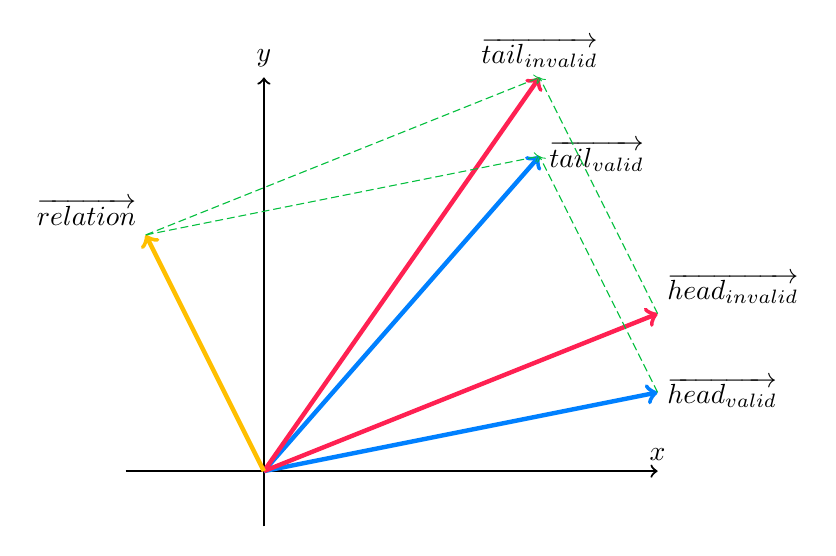
\begin{tikzpicture}[
		arrow/.style={->,thick},
		vector/.style={arrow, ultra thick},
		dashLine/.style={->, thin, dash pattern=on 1mm off 0.5mm},
		formal/.style={font=\sffamily}]
		\coordinate (root) at (0,0);
		\coordinate [formal, label=above left:$\overrightarrow{\text{relation}}$] (c1) at (-1.5, 3);
		\coordinate [formal, label=above:$\overrightarrow{\text{tail}_{\text{invalid}}}$] (c2) at (3.5, 5);
		\coordinate [formal, label=right:$\overrightarrow{\text{tail}_{\text{valid}}}$] (c3) at (3.5, 4);
		\coordinate [formal, label=above right :$\overrightarrow{\text{head}_{\text{invalid}}}$] (c4) at (5, 2);
		\coordinate [formal, label=right:$\overrightarrow{\text{head}_{\text{valid}}}$] (c5) at (5, 1);
		
		\draw [arrow] ([yshift=-2em] root) -> (0, 5) node (yaxis)[above] {$y$};
		\draw [arrow] ([xshift=-5em] root) -> (5, 0) node (xaxis)[above] {$x$};
		
		\foreach \x in {3, 5}
		{\draw [vector, color=azure] (root) -> (c\x);}
		
		\foreach \x in {2, 4}
		{\draw [vector, color=awesome] (root) -> (c\x);}
		
		\draw [vector, color=amber] (root) -> (c1);
		
		\foreach \x in {1, 4}
		{\draw [dashLine, color=darkpastelgreen] (c\x) -> (c2);}
		
		\foreach \x in {1, 5}
		{\draw [dashLine, color=darkpastelgreen] (c\x) -> (c3);}
	\end{tikzpicture}
	\caption{Minh họa về các vector nhúng trong mô hình TransE}
	\label{fig:TransEAnimation}
\end{figure}

Tương tự như phương pháp Word2Vec\cite{mikolov2013efficient}, mô hình \textit{Biến đổi vector nhúng để mô hình hóa dữ liệu đa-quan hệ} (TransE \cite{bordes2013translating}) thuộc nhóm các phương pháp nhúng hình học để biến đổi các thực thể thể và quan hệ trong đồ thị tri thức thành các vector nhúng đầu ra sao cho :
\begin{equation}
\label{eq:conditionTransE}
\overrightarrow{\text{entity}_{\text{head}}} + \overrightarrow{relation} \approx \overrightarrow{\text{entity}_{\text{tail}}}
\end{equation}

Đầu tiên, các vector nhúng thực thể và quan hệ được khởi tạo ngẫu nhiên bằng phân phối chuẩn theo số chiều của vector khởi tạo $D_{\text{in}}$, sau đó được chuẩn hóa theo kích thước của tập thực thể nhúng, và quan hệ nhúng.
Sau đó, ta lấy mẫu (sampling) từ tập dữ liệu huấn luyện để có được một \textit{lô bộ ba hợp lệ} ($S_{\text{batch}}$). Với mỗi bộ ba như vậy, chúng ta lấy mẫu bộ ba không hợp lệ bằng cách thay thực thể đầu hoặc thực thể đuôi bằng một thực thể ngẫu nhiên trong tập thực thể để được \textit{lô bộ ba không hợp lệ} ($S'_{\text{batch}}$). Sau đó ta nhóm từng bộ ba hợp lệ với không hợp lệ để tạo ra \textit{lô huấn luyện} ($T_{\text{batch}}$). Cuối cùng, ta cập nhật giá trị các vector nhúng để đảm bảo điều kiện \ref{eq:conditionTransE}.

Mô hình TransE của nhóm tác giả Bordes, Antoine\cite{bordes2013translating} được trình bày ở thuật toán \ref{alg:TransE} như sau :

\begin{algorithm}
	\caption{Thuật toán học vector nhúng TransE}\label{alg:TransE}
	\begin{algorithmic}[1]
		\Statex \textbf{Input} : 
		Tập huấn luyện $S = {(h, r, t)}$, tập thực thể E, tập quan hệ R, biên lề $\gamma$, số chiều nhúng $D_{\text{in}}$
		\Statex \textbf{Initialize}
		\State $\overrightarrow{r} \leftarrow \text{uniform}(-\frac{6}{\sqrt{D_{\text{in}}}}, \frac{6}{\sqrt{D_{\text{in}}}})$ với mỗi quan hệ $r \in R$
		\State $\overrightarrow{r} \leftarrow \overrightarrow{r}/\|\overrightarrow{r}\|$ với mỗi $r \in R$
		\State $\overrightarrow{e} \leftarrow \text{uniform}(-\frac{6}{\sqrt{D_{\text{in}}}}, \frac{6}{\sqrt{D_{\text{in}}}})$ với mỗi thực thể $e \in E$
		\Loop
		\State $\overrightarrow{e} \leftarrow \overrightarrow{e}/\|\overrightarrow{e}\|$ với mỗi $e \in E$
		\State $S_{\text{batch}} \leftarrow \text{sample}(S, b)$  // lấy mẫu minibatch kích thước $b$
		\State $T_{\text{batch}} \leftarrow \varnothing $
		\For {$(h, r, t) \in S_{\text{batch}}$}
		\State $(h', r, t') \leftarrow \text{sample}(S'_{(h, r, t)})$ // lấy mẫu từ bộ ba không hơp lệ
		\State $T_{\text{batch}} \leftarrow T_{\text{batch}} \cup \Big\{ \Big( (h, r, t), (h', r, t') \Big) \Big\}$
		\EndFor
		\Statex Cập nhật nhúng
		\State $\sum_{\Big( (h, r, t), (h', r, t')\Big) \in T_{\text{batch}}} \nabla [\gamma + d(\overrightarrow{h} + \overrightarrow{r}, \overrightarrow{t}) - d(\overrightarrow{h'} + \overrightarrow{r}, \overrightarrow{t'})]_{+}$
		\EndLoop
	\end{algorithmic}
\end{algorithm}

Trong đó, đầu vào của mô hình TransE là tập dữ liệu huấn luyện với mỗi phần tử là một bộ ba $(h, r, t)$. $h, t \in E$ là các thực thể đầu và thực thể đuôi, $r \in R$ là các quan hệ.$\overrightarrow{e}$ và $\overrightarrow{r}$ lần lượt là các vector nhúng của thực thể và quan hệ, và $\|\overrightarrow{e}\|$ và $\|\overrightarrow{r}\|$ lần lượt là độ lớn của tập thực thể và tập quan hệ. $S$ và $S_{\text{batch}}$ tương ứng là tập dữ liệu huấn luyện, và một lô (batch) lấy ra từ tập dữ liệu huấn luyện.
$T_{\text{batch}}$ là một lô bao gồm cả bộ ba hợp lệ và bộ ba không hợp lệ để tính hàm mất mát \ref{eq:lossTransE}

Trong đó \textit{bộ ba hợp lệ} (valid triple) là bộ ba lấy từ lô huấn luyện ($S_{\text{batch}}$), \textit{bộ ba không hợp lệ} (invalid triple) là bộ ba lấy từ lô huấn luyện lỗi ($S'_{\text{batch}}$) được bỏ đi thực thể đầu hoặc thực thể đuôi và thay thế các thực thể đó bằng cách chọn một thực thể ngẫu nhiên trong tập thực thể :

\begin{equation}
	\label{eq:lossTransE}
	\centering
	S'_{(h, r, t)} = \big\{ (h', r, t) | h' \in E \big\} \cup \big\{ (h, r, t') | t' \in E \big\}
\end{equation}

Để đạt được mục tiêu là tạo ra các vector nhúng sao cho $\overrightarrow{h} + \overrightarrow{r} \approx \overrightarrow{t}$, ý tưởng của mô hình là các vector nhúng trong lô hợp lệ thì vector nhúng đuôi $\overrightarrow{t}$ phải ở lân cận của $\overrightarrow{h} + \overrightarrow{r}$, ngược lại các vector nhúng trong lô không hợp lệ $\overrightarrow{h'} + \overrightarrow{r}$ (hoặc $\overrightarrow{t'}$) thì phải nằm xa so với $\overrightarrow{t}$ (hoặc $\overrightarrow{h} + \overrightarrow{r}$) theo hàm mất mát sau :

\begin{equation}
 \label{eq:KBGATLoss}
	\centering
	\mathcal{L} = \sum_{(h, r, t) \in S} \sum_{(h', r, t') \in S'_{(h, r, t)}} [\gamma + d(\overrightarrow{h}+ \overrightarrow{r}, \overrightarrow{t}) - d(\overrightarrow{h'}+ \overrightarrow{r}, \overrightarrow{t'})]_{+}
\end{equation}

Với $\gamma > 0$ là biên lề, và $[x]_{+}$ là lấy phần dương của $x$. $d$ là đo giá trị sai khác của các thực thể nhúng trong lô hợp lệ và lô không hợp lệ :

$$d(\overrightarrow{h} + \overrightarrow{r}, \overrightarrow{t}) = \big\| \overrightarrow{h} + \overrightarrow{r} - \overrightarrow{t}\big\|_{p}$$

Hàm $\|\|_{p}$ là hàm chuẩn hóa có thể là L1-norm (p = 1) hoặc L2-norm (p = 2).

\subsection{Mô hình nhúng KBGAT}
\label{sec:encodeKBGAT}

Sau khi có được các vector nhúng học được các đặc trưng không gian ở trên của đồ thị. Các vector nhúng tiếp tục được đi qua lớp nhúng tiếp theo để tổng hợp thêm thông tin lân cận của một thực thể.

\definecolor{amber}{rgb}{1.0, 0.75, 0.0}
\definecolor{azure}{rgb}{0.0, 0.5, 1.0}
\definecolor{awesome}{rgb}{1.0, 0.13, 0.32}
\definecolor{deepskyblue}{rgb}{0.0, 0.75, 1.0}
\definecolor{deepmagenta}{rgb}{0.8, 0.0, 0.8}
\definecolor{deepcarminepink}{rgb}{0.94, 0.19, 0.22}
\definecolor{gray}{rgb}{0.5, 0.5, 0.5}
\begin{figure}[htp]
	\centering
	\resizebox{\textwidth}{!}{%
		\begin{tikzpicture}[
			emb/.style={draw, circle,minimum width=.1em, thin, anchor=center},
			entityInit/.style={emb, fill=amber},
			relationInit/.style={emb, fill=azure},
			entityEmb/.style={emb, fill=gray},
			relationEmb/.style={emb, fill=deepcarminepink},
			entityPretrain/.style={emb, fill=deepmagenta},
			entityOut/.style={emb, fill=deepskyblue},
			box/.style={draw,rectangle, fill=none},
			embBox/.style={box ,rounded corners=0.2em, minimum width=1.3em},
			layerBox/.style={color=azure!80, box ,very thick,rounded corners=0.2em, minimum width=1.3em},
			textbox/.style={box,rounded corners=0.3em, fill=none,font=\sffamily, align=center},
			arrowStrong/.style={thick,->,>=stealth},
			arrowDash/.style={thick, ->,>=stealth, dash pattern=on 1.5mm off 0.7mm, postaction={decorate}},
			row/.style={draw, rectangle, font=\fontsize{0.6em}{1}\sffamily, align=center, text width=3.9em},
			arrowStyle/.style={-latex', font=\sffamily},
			mydot/.style={draw, circle, minimum size=0.1em, scale=0.2},
			]
			% 5
			% Root
			\draw node[textbox][text width=5.7em] (graphAttention2) {\small Graph Attention Layer $2_{\ref{eq:graphAttention2}}$};
			
			\draw node[textbox][minimum width=9.5em, minimum height=21em, left=1.5em of graphAttention2] (layer3) {};
			
			\draw node[embBox][minimum height=20.3em, left=2em of graphAttention2] (box10) {};
			\begin{scope}[every node/.style={below=0mm of box10.center}]
				\foreach \x in {1,...,12}
				{\draw node[entityEmb][yshift=(\x-4)*1.1em+0.55em] (ex10\x) {};}
				
				\foreach \x in {1,...,6}
				{\draw node[relationEmb](ey10\x)[yshift=-(\x+3)*1.1em+0.55em]{};}
			\end{scope}
			
			\draw node[embBox][minimum height=7em, left=2em of box10, yshift=5em] (box7) {};
			\draw node[embBox][minimum height=7em, left=2em of box10, yshift=-5em] (box9) {};
			\begin{scope}
				\foreach \x in {1,...,6}
				{\draw node[entityEmb](e7\x)[yshift=(\x-3)*1.1em, below=0mm of box7.center]{};}
				
				\foreach \x in {1,...,6}
				{\draw node[relationEmb](e9\x)[yshift=(\x-3)*1.1em, below=0mm of box9.center]{};}
			\end{scope}
			
			\draw node[embBox][minimum height=4em, left=2em of box7, yshift=2.5em] (box5) {};
			\draw node[embBox][minimum height=4em, left=2em of box7, yshift=-2.5em] (box6) {};
			\draw node[embBox][minimum height=5em, left=2em of box9] (box8) {};
			\begin{scope}
				\foreach \x in {1,...,3}
				{\draw node[entityEmb](e5\x)[yshift=(\x-2)*1.1em+0.55em, below=0mm of box5.center]{};}
				
				\foreach \x in {1,...,3}
				{\draw node[entityEmb](e6\x)[yshift=-(\x-2)*1.1em+0.55em, below=0mm of box6.center]{};}
				
				\foreach \x in {1,...,4}
				{\draw node[relationInit](e8\x)[yshift=(\x-2)*1.1em, below=0mm of box8.center]{};}
			\end{scope}
			\draw node[layerBox][minimum height=8em,minimum width=5.5em, left=1.5em of box10, yshift=-5em] (fc1) {};
			
			% Left
			\begin{scope}[every node/.style={left=2em of layer3}]
				\draw node[textbox][yshift=3em, text width=3em] (attentionHead1) {\small Attention Head 1};
				\draw node[textbox][yshift=-3em, text width=3em] (attentionHead2) {\small Attention Head 2};
			\end{scope}
			\draw node[textbox][left=1.5em of layer3, text width=4em, minimum width=4em, minimum height=10em] (graphAttention1) {\small Graph Attention Layer $1_{\ref{eq:graphAttention1}}$ };
			
			\draw node[textbox][minimum width=12.3em, minimum height=21em, left=1.5em of graphAttention1] (layer1) {};
			% Layer 1
			\draw node[embBox][minimum height=10.5em, yshift=1em,right=3em of layer1.center, left=2em of graphAttention1] (box4) {};
			\begin{scope}
				\foreach \x in {1,...,6}
				{\draw node[entityInit](ex4\x)[yshift=(\x-2)*1.1em-0.4em, above=0em of box4.center]{};}
				
				\foreach \x in {1,...,3}
				{\draw node[relationInit](e4y\x)[yshift=-(\x)*1.1em-0.6em, below=0mm of box4.center]{};}
			\end{scope}
			
			% Start Initial
			\draw node[embBox][minimum height=4em, yshift=4.5em, left=2em of box4] (box1) {};
			\foreach \x in {1,...,3}
			{\draw node[entityInit](e1\x)[yshift=(\x-2)*1.1em+0.5em, below=0mm of box1.center]{};}
			
			\draw node[embBox][minimum height=4em, left=2em of box4] (box2) {};
			\foreach \x in {1,...,3}
			{\draw node[relationInit](e2\x)[yshift=(\x-2)*1.1em+0.5em, below=0mm of box2.center]{};}
			
			\draw node[embBox][minimum height=4em, yshift=-4.5em, left=2em of box4] (box3) {};
			\foreach \x in {1,...,3}
			{\draw node[entityInit](e3\x)[yshift=(\x-2)*1.1em+0.5em, below=0mm of box3.center]{};}
			% Start Initial
			
			\begin{scope}[every node/.style={left=of box2, row}]
				\draw node (relation1) {president\_of};
				\draw node[above=0mm of relation1] (entity1) {Donald Trump};
				\draw node[above=0mm of entity1] (triple1) {Triple 1};
				\draw node[below=0mm of relation1] (entity2) {United States};	
			\end{scope}
			
			\begin{scope}[every node/.style={row}]
				\draw node[below=3em of entity2] (triple2) {Triple N};
				\draw node[below=0mm of triple2] (entity3) {Tom Cruise};
				\draw node[below=0mm of entity3] (relation2) {born\_in};
				\draw node[below=0mm of relation2] (entity4) {New York};	
			\end{scope}
			
			% Right
			\draw node[textbox][minimum height=16em, minimum width=2.3em, yshift=-4em, right=1.5em of graphAttention2] (layer4){};
			\draw node[embBox][minimum height=7em, right=2em of graphAttention2] (box11) {};
			\begin{scope}
				\foreach \x in {1,...,6}
				{\draw node[entityEmb](e11\x)[yshift=(\x-3)*1.1em, below=0mm of box11.center]{};}
			\end{scope}
			
			\draw node[embBox][minimum height=7em, below=0.7em of box11] (box12) {};
			\begin{scope}
				\foreach \x in {1,...,6}
				{\draw node[relationEmb](e12\x)[yshift=(\x-3)*1.1em, below=0mm of box12.center]{};}
			\end{scope}
			
			\draw node[embBox][minimum height=7em, above=1.5em of box11] (box13) {};
			\begin{scope}
				\foreach \x in {1,...,6}
				{\draw node[entityPretrain](e13\x)[yshift=(\x-3)*1.1em, below=0mm of box13.center]{};}
			\end{scope}
			
			\draw node[embBox][minimum height=5em, left=1.7em of box13] (box14) {};
			\begin{scope}
				\foreach \x in {1,...,4}
				{\draw node[entityInit](e14\x)[yshift=(\x-2)*1.1em, below=0mm of box14.center]{};}
			\end{scope}
			\draw node[layerBox][minimum height=8em, minimum width=5.5em, above=1.5em of box11, yshift=-0.5em, xshift=-1.5em] (fc2) {};
			
			\draw node[right=2em of box11, yshift=3.7em] (bigOTimes) {$\bigotimes^{\ref{eq:reInitEmbedding}}$};
			
			\draw node[textbox][minimum height=16em, minimum width=2.3em, yshift=-3.95em, right=1.5em of bigOTimes] (layer5) {};
			\draw node[embBox][minimum height=7em, above=1em of layer5.center, yshift=-0.5em] (box15) {};
			\begin{scope}
				\foreach \x in {1,...,6}
				{\draw node[entityOut](e15\x)[yshift=(\x-3)*1.1em, below=0mm of box15.center]{};}
			\end{scope}
			
			\draw node[embBox][minimum height=7em, below=1em of layer5.center, yshift=0.5em] (box16) {};
			\begin{scope}
				\foreach \x in {1,...,6}
				{\draw node[relationEmb](e16\x)[yshift=(\x-3)*1.1em, below=0mm of box16.center]{};}
			\end{scope}
			
			\draw node[textbox][right=1.5em of layer5] (final) {$\mathcal{L}_{\ref{eq:KBGATLoss}}$};
			%16
			% Arrow
			\draw [arrowStrong] (box10) -- (graphAttention2.west);
			
			\draw [arrowStrong] (entity1.east) -- (box1.west);
			\draw [arrowStrong] (relation1) -- (box2.west);
			\draw [arrowStrong] (entity2.east) -- (box3.west);
			
			\draw [arrowStrong] (graphAttention2.east) -- (box11.west);
			\draw [arrowStrong] (graphAttention2.east) -- (box12.west);
			
			\draw [arrowStrong] (box11.east) to ([xshift=0.35em] bigOTimes.west);
			\draw [arrowStrong] (box13.east) to ([xshift=0.35em] bigOTimes.west);
			
			\draw [arrowStrong] ([xshift=-1.7em] bigOTimes.east) -- (box15.west);
			
			\draw [arrowStrong] (box16.east) -- (final.west);
			\draw [arrowStrong] (box15.east) -- (final.west);
			
			\foreach \x in {1,2}
			\draw [arrowStrong] (layer1.east) -- (attentionHead\x.west);
			
			\foreach \x in {1,2}
			\draw [arrowStrong] (attentionHead\x.east) -- (layer3.west);
			
			\foreach \x in {1,2,3}
			\draw [arrowDash] (box\x.east) -- (box4.west);
			
			\foreach \x in {7,9}
			{\draw [arrowDash] (box\x) -- (box10.west);}
			
			\foreach \x in {5,6}
			{\draw [arrowDash] (box\x) -- (box7.west);}
			
			\foreach \x in {1, ..., 6}
			{\draw [thick] (e81) -- (e9\x);}
			\foreach \x in {1, ..., 6}
			{\draw [thick] (e82) -- (e9\x);}
			\foreach \x in {1, ..., 6}
			{\draw [thick] (e83) -- (e9\x);}
			\foreach \x in {1, ..., 6}
			{\draw [thick] (e84) -- (e9\x);}
			
			\foreach \x in {1, ..., 6}
			{\draw [thick] (e141) -- (e13\x);}
			\foreach \x in {1, ..., 6}
			{\draw [thick] (e142) -- (e13\x);}
			\foreach \x in {1, ..., 6}
			{\draw [thick] (e143) -- (e13\x);}
			\foreach \x in {1, ..., 6}
			{\draw [thick] (e144) -- (e13\x);}
			
			%		\foreach \x in {1, ..., 6}
			%		{\draw [thick] (r34) -- (r1\x);}
			
			\draw node[mydot][below=1.1em of entity2] (dot1) {};
			\draw node[mydot][below=1.4em of entity2] (dot2) {};
			\draw node[mydot][below=1.7em of entity2] (dot3) {};
		\end{tikzpicture}
	}
	\caption{Minh họa các lớp mã hóa của mô hình KBGAT}
	\label{fig:encoderKBGAT}
\end{figure}

Mô hình sẽ biến đổi từ ma trận nhúng thực thể

$\mathbf{E} = \Big\{\overrightarrow{e_1}, \overrightarrow{e_2}, ...,  \overrightarrow{e_{N_e}}\Big\} \xrightarrow{} \mathbf{E''} = \Big\{\overrightarrow{e''_1}, \overrightarrow{e''_2}, ...,  \overrightarrow{e''_{N_e}}\Big\}$, với $\mathbf{E} \in \mathbb{R}^{N_e \times D_{\text{in}}}$ và $\mathbf{E''} \in \mathbb{R}^{N_e \times D''}$.
Đồng thời biến đổi ma trận nhúng quan hệ 
$\mathbf{R} = \Big\{\overrightarrow{r_1}, \overrightarrow{r_2}, ...,  \overrightarrow{r_{N_r}}\Big\} \xrightarrow{} \mathbf{R''} = \Big\{\overrightarrow{r''_1}, \overrightarrow{r''_2}, ...,  \overrightarrow{r''_{N_r}}\Big\}$ với $\mathbf{R} \in \mathbb{R}^{N_r \times P_{\text{in}}}$ và $\mathbf{R''} \in \mathbb{R}^{N_r \times P''}$. Tương tự như mô hình GAT đã trình bày ở mục \ref{sec:GAT}, mô hình sẽ biến đổi vector nhúng thực thể $D_{\text{in}}$ chiều thành $D''$ chiều với thông tin được tổng hợp từ các hệ số chú ý lân cận. $P_{\text{in}}$ và $P''$ lần lượt là số chiều của vector nhúng quan hệ đầu vào và đầu ra. $N_e$, $N_r$ tương ứng là kích thước của tập thực thể và tập quan hệ trong $\mathcal{G}_{know}$.

Mô hình KBGAT sẽ ghép các vector nhúng thực thể và vector nhúng quan hệ theo cấu trúc như sau :

\begin{equation}
\label{attentionWithRelation}
\overrightarrow{t_{ijk}} = \mathbf{W_1} [\overrightarrow{e_i} || \overrightarrow{e_j} || \overrightarrow{r_k}]
\end{equation}

Với $\overrightarrow{t_{ijk}}$ là vector nhúng đại diện cho bộ ba  $t_{ij}^k = (e_i, r_k, e_j)$ với $e_j$, và $r_k$ lần lượt là các thực thể hàng xóm và quan hệ nối giữa đỉnh gốc $e_i$ với đỉnh $e_j$ , $\mathbf{W} \in \mathbb{R}^{D_k \times (2 D_{\text{in}} + P_{\text{in}})}$ là ma trận trọng số thể hiện quá trình biến đổi tuyến tính từ các vector đã ghép lại với nhau thành một vector với số chiều $D_k$ mới. Các ma trận trọng số trên được khởi tạo ngẫu nhiên theo phân phối chuẩn hoặc tái huấn luyện (pre-train) bằng mô hình TransE \cite{bordes2013translating}.

Tương tự với công thức \ref{attentionCoeff} của mô hình GAT, ta cần tính hệ số chú ý của từng cạnh đối với từng đỉnh, sau đó áp dụng hàm \textit{softmax} để chuẩn hóa hệ số lại theo công thức sau :

\begin{equation}
\label{attentionRelationCoeff}
\begin{split}
\alpha_{ijk}& = \text{softmax}_{jk}(\text{LeakyReLU}(\mathbf{W_2} \overrightarrow{t_{ijk}}))\\
&= \frac{
	\text{exp} \Big( \text{LeakyReLU} \Big( \mathbf{W_2} \overrightarrow{t_{ijk}}\Big) \Big))
}
{
	\sum_{n\in \mathcal{N}_i} \sum_{r\in \mathcal{R}_{in}}
	\text{exp} \Big( \text{LeakyReLU} \Big( \mathbf{W_2} \overrightarrow{t_{inr}} \Big) \Big)
}
\end{split}
\end{equation}

%Trong đồ thị, mỗi cạnh của thực thể không chỉ được biểu diễn thông tin bởi thực thể đầu $e_\text{head}$ và thực thể đích $e_\text{tail}$ mà có các quan hệ giữa chúng. Hơn nữa trong một cạnh, các thực thể còn có thể đóng nhiều vai trò khác nhau phụ thuộc vào các loại quan hệ khác nhau. Vì vậy phương pháp KBGAT bổ sung thêm thông tin của một vector nhúng quan hệ vào một cạnh  nhúng $(\overrightarrow{e_\text{i}}, \overrightarrow{r_k}, \overrightarrow{e_\text{j}})$. Tuy nhiên một vector $\overrightarrow{e_i}$ hay $\overrightarrow{r_k}$ không thể biểu thị một cách đầy đủ tri thức của một thực thể $e_i$ hay quan hệ $r_k$ trong một đồ thị, vì một tri thức sẽ có thể có mối liên hệ với những tri thức lân cận hay nói cách khác một \textbf{thực thể nhúng} (entity embedding) hay một \textbf{quan hệ nhúng} (relation embedding) sẽ cần thêm thông tin của các vector nhúng của thực thể lân cận và quan hệ lân cận khác để có thể là một đại diện đầy đủ . Chính vì vậy phương pháp \textit{n-hop neighborhood} \cite{lin2018multi} sẽ giúp bổ sung thêm thông tin lân cận của thực thể $e_i$ và quan hệ $r_k$ bằng cách ghép chồng để tạo thành một vector mới theo công thức sau :
%\begin{align}
%{\overrightarrow{h_i} = [\overrightarrow{e_i} \bigparallel_{\text{axis}=1} \overrightarrow{e_{i_{\text{n-hop}}}}]} \hspace{0.5cm};\hspace{1.5cm}&
%{\overrightarrow{g_k} = [\overrightarrow{r_k} \bigparallel_{\text{axis}=1} \overrightarrow{r_{k_{\text{n-hop}}}}]}
%\end{align}
%
%Trong đó $\overrightarrow{h_i}$, $\overrightarrow{g_k}$ tương ứng là vector nhúng mới của thực thể $e_i$ và các thực thể lân cận ($e_{i_{\text{n-hop}}}$) hay quan hệ $r_k$ và các quan hệ lân cận ($r_{k_{\text{n-hop}}}$); ký hiệu $\bigparallel_{\text{axis}=1}$ biểu thị cho phép xếp chồng lên nhau. Các vector $\overrightarrow{e_{i_{\text{n-hop}}}}$ và $\overrightarrow{r_{k_{\text{n-hop}}}}$ được tính bằng tổng vector nhúng của các thực thể hoặc các quan hệ lân cận đi qua $n-hop$ độ sâu bắt đầu từ $e_i$ theo công thức sau : 
%
%\begin{align}
%{\overrightarrow{e_{i_{\text{n-hop}}}} = \bigparallel_{d=1}^{\text{n-hop}} \sum_{n \in \mathcal{N}_i} \overrightarrow{e_n^d}} \hspace{0.5cm};\hspace{1.5cm}&
%{\overrightarrow{r_{k_{\text{n-hop}}}} = \bigparallel_{d=1}^{\text{n-hop}} \sum_{m \in \mathcal{N}_k} \overrightarrow{r_m^d}}
%\end{align}
%
%Với mối thực thể $e_n$ hay quan hệ $r_m$ có độ sâu d (depth) bắt đầu từ thực thể $e_i$, ta sẽ tính tổng các vector nhúng và ghép chồng với nhau.
%
%Để biểu thị cho quá trình biến tuyến tính của vector nhúng, ta cho mỗi vector nhúng đi qua một ma trận trọng số : $\overrightarrow{h'_i} = \mathbf{W}_{\text{entity}} \overrightarrow{h_i}$ 
%và $\overrightarrow{g'_i} = \mathbf{W}_{\text{relation}} \overrightarrow{g_i}$. Tuy nhiên để thu được một trọng số mới biểu diễn bộ ba $t^k_{ij} = (e_{\text{head}}, relation, e_{\text{tail}})$ tương ứng với một cạnh trong trong KB. Ta thực hiện quá trình biến đổi tuyến tính đó bằng cách ghép cả thực thể và mối quan hệ với nhau rồi nhân với một ma trận trọng số chung như công thức sau :
%
%trong đó $\overrightarrow{t_{ijk}}$ là một vector nhúng biểu diễn cho một bộ ba $t^k_{ij}$. Các vector $\overrightarrow{h_i}$, $\overrightarrow{h_j}$ và $\overrightarrow{g_j}$ tương ứng là vector nhúng của các thực thể $e_i$, $e_j$ và quan hệ $r_k$. $\mathbf{W_1} \in \mathbb{R}^{3 T \times S^\text{batch}}$ . Để áp dụng cơ chế chú ý (attention mechanisms \cite{vaswani2017attention}), ta cần học sự quan trọng của một cạnh $t_{ij}^k$ bởi giá trị của $b_{ij}^k$. Để tham số hóa quá trình biến đổi tuyến tính ta nhân với ma trận trọng số $\mathbb{W}_{2}$ và lấy giá trị chú ý tuyệt đối bằng hàm $LeakyRelu$ theo công thức sau :
%
%\begin{align}
%b_{ijk} = \text{LeakyRelu}\Big( \mathbf{W_2} t_{ijk} \Big)
%\end{align}
%
%Sau đó, với mỗi độ lớn của $b^k_{ij}$ được cho qua hàm \textit{softmax} để tính giá trị thể hiện xác xuất của từng giá trị chú ý $\alpha_{ijk}$ đối với từng bộ ba .

trong đó $\mathcal{N}_i$ là tập hợp hàng xóm của đỉnh gốc $e_i$ có độ sâu $n_{\text{hop}}$; $\mathcal{R_{\textit{i} \textit{n}}}$ là tập hợp tất cả những quan hệ nằm trên đường đi (path) từ thực thể gốc $e_i$ với thực thể $e_n \in \mathcal{N}_i$. Tương tự công thức \ref{scaleAttentionCoef}, các vector nhúng $\overrightarrow{t^k_{ij}}$ sẽ được thu nhỏ hoặc mở rộng khi nhân với hệ số chú ý đã được chuẩn hóa :

\begin{align}
{\overrightarrow{e'_{i}}}&={\sigma\left(\sum_{j \in \mathcal{N}_i} \sum_{k \in \mathcal{R}_{ij}} \alpha_{ijk} \overrightarrow{t_{ijk}}\right)}
\end{align}

Tương tự như công thức \ref{multiHeadAttention} của \textit{cơ chế mặt nạ chú ý}, ta sẽ ghép $N_{\text{head}}$ đỉnh chú ý lại với nhau để ổn định quá trình học :

\begin{equation}
\label{eq:graphAttention1}
\overrightarrow{e'}_i=\bigparallel_{h=1}^{N_{\text{head}}} \sigma\left(\sum_{j\in \mathcal{N}_i}\alpha_{ijk}^{(h)} \overrightarrow{t^{(h)}_{ijk}}\right)
\end{equation}

Tương tự như các vector nhúng thực thể, các vector nhúng quan hệ cũng được nhân với một ma trận trọng số $\mathbf{W}_R$ để thực hiện biến đổi tuyến tính các vector nhúng quan hệ $P$ chiều lên vector nhúng có $P'$ chiều :

\begin{align}
\mathbf{R'} = \mathbf{R} \mathbf{W}^R; \hspace{2cm} \text{với: } \mathbf{W}^R \in \mathbb{R}^{P \times P'}
\end{align}

Đến đây, ta đã có hai ma trận $\mathbf{H}' \in \mathbb{R}^{N_e \times D'}$ và $\mathbf{R}' \in \mathbb{R}^{N_r \times P'}$ tương ứng là ma trận quan hệ và ma trận thực thể với số chiều mới. Mô hình sẽ đi qua lớp chú ý cuối cùng với đầu vào các vector nhúng quan hệ và thực thể mới như \ref{multiHeadConcat} . Tuy nhiên, nếu chúng ta thực hiện chú ý đa đỉnh trên lớp cuối cùng này để dự đoán, phép ghép chồng sẽ không còn \textit{nhạy cảm} với cơ chế tự-chú ý. Vì vậy thay vì ghép chồng, mô hình sẽ tính trung bình và sau đó áp dụng hàm phi tuyến tính cuối cùng :

\begin{equation}
\label{eq:graphAttention2}
\overrightarrow{e''_{i}}=\sigma\left(\frac{1}{N_{\text{head}}} \sum_{h=1}^{N_{\text{head}}} \sum_{j \in \mathcal{N}_i} \sum_{k \in \mathcal{R}_{ij}} \alpha'^{(h)}_{ijk} \overrightarrow{t'^{(h)}_{ijk}} \right)
\end{equation}

Với $\alpha'^{(h)}_{ijk}$ và $t'^{(h)}_{ijk}$ tương ứng là hệ số chú ý đã chuẩn hóa và vector nhúng đại diện cho một bộ ba $(e_i, r_k, e_j)$ thuộc các lớp $(h)$ khác nhau.

Đến đây, mô hình KBGAT đã áp dụng giống như mô hình GAT \ref{sec:GAT} nhưng ta bổ sung thêm thông tin vector nhúng thực thể và thông tin các đỉnh hàng xóm cách $n_{\text{hop}}$ bậc, ta đã thu được ma trận nhúng thực thể $\mathbf{E}'' \in \mathbb{R}^{N_e \times D''}$, và ma trận nhúng quan hệ $\mathbf{R}'' \in \mathbb{R}^{N_r \times P''}$. Tuy nhiên, sau khi trải qua quá trình học ma trận nhúng mới, ma trận nhúng thực thể $\mathbf{E}''$ mất đi thông tin nhúng khởi tạo ban đầu. Để giải quyết vấn đề này, mô hình sẽ cho nhân ma trận nhúng khởi tạo ban đầu $\mathbf{E}$ với một ma trận trọng số $\mathbf{W}^E \in \mathbb{R}^{D_{\text{in}} \times D''}$ để tạo thành ma trận nhúng mới rồi cộng trực tiếp ma trận nhúng đó vào để đảm bảo thông tin nhúng khởi tạo trong quá trình huấn luyện :

\begin{equation}
\label{eq:reInitEmbedding}
\mathbf{H} = \mathbf{W}^E \mathbf{E} + \mathbf{E''}
\end{equation}

Cuối cùng, các bộ dữ liệu huấn luyện sẽ được lấy mẫu để tạo ra bộ ba hợp lệ (valid triple), và bộ ba không hợp lệ (invalid triple) tương tự như mô hình TransE được trình bày ở trên để học được các vector nhúng.
Tuy nhiên công thức tính sự khác biệt giữa các vector nhúng được chuẩn hóa L1 theo công thức sau  :
$d_{t_{ij}} = \big|\big|\vec{h_i}+ \vec{g_k}-\vec{h_j}\big|\big|_1$.

Tương tự, chúng tôi huấn luyện sử dụng hàm mất mát-lề :

\begin{equation}
L(\Omega)=\sum_{t_{ij} \in S} \sum_{t'_{ij} \in S'} \text{max}\{d_{t'_{ij}} - d_{t_{ij}} + \gamma , 0 \}
\end{equation}

trong đó $\gamma > 0$ là tham số lề, $S$ là tập hợp bộ ba chuẩn (valid triple), và $S'$ là tập hợp của ba lỗi (invalid triple) theo công thức sau :

\begin{equation}
{S'} ={\underbrace{\{ t^k_{i'j} | e'_i \in \mathcal{E}\setminus e_i\}}_{\text{thay thế thực thể đầu}}\cup \underbrace{\{ t^k_{ij'} | e'_j \in \mathcal{E}\setminus e_j\}}_{\text{thay thế thực thể đuôi}}}
\end{equation}

\subsection{Dự đoán}
\label{sec:predictionConvKB}

Sau khi chúng ta biểu diễn các thực thể và quan hệ lên không gian số chiều thấp, mô hình sẽ sử dụng \cite{nguyen2017novel} làm mô hình để phân tích các đặc trưng toàn cục của một bộ ba $t_{ijk}$ qua mỗi chiều để khái quát hóa các đặc trưng biến đổi của mô hình bằng các lớp tính tích chập. Hàm tính điểm số với những ánh xạ đặc trưng được tính theo công thức sau :

\begin{equation}
f(t_{i j k}) = \Big( \bigparallel_{m=1}^{\Omega} \text{ReLU} ([\overrightarrow{e_i}, \overrightarrow{r_k}, \overrightarrow{h_j}] \ast \omega^m)\Big).\mathbf{W}
\end{equation}

trong đó $\omega^m$ thể hiện bộ lọc tích chập thứ $m-th$,
\(\omega\) là siêu tham số về số lượng lớp tích chập, \(\ast\) là thao tác thực hiện tính tích chập, và \(\mathbf{W} \in \mathbb{R}^{\Omega k \times 1}\)
biểu thị ma trận biến đổi tuyến tính được sử dụng để tính kết quả cuối cùng của bộ ba. Mô hình được huấn luyện bằng lề-mềm (soft-margin) như sau :

\begin{equation}
\mathcal{L} = \sum_{t^k_{ij} \in \{S \cup S'\}} \text{log}(1 + exp(l_{t^k_{ij}} . f(t^k_{ij}))) + \frac{\lambda}{2} \parallel{\mathbf{W}}\parallel_2^2
\end{equation}
trong đó $l_{t^k_{ij}} = \begin{cases}
1 &\text{for } t^k_{ij} \in S \\
-1 &\text{for } t^k_{ij} \in S' \\
\end{cases}$

